\flushbottom

%%
%% Prove the assertion in the paragraph before the result on Fredholm Alt. Thrm.
%%
%% Consider adding  a section on Modified Green Functions.
%%
%% Before presenting the Fredholm alternative theorem.  Do the analogous 
%% work for the inhomogeneous matrix equation.  State the existence, 
%% uniqueness results for Ax=b in terms of the eigenvectors of A.
%%




%%============================================================================
%%============================================================================
\chapter{Inhomogeneous Differential Equations}
\label{chapter_io}

Feelin' stupid?  I know I am!

\begin{flushright}
  -Homer Simpson
\end{flushright}








%%============================================================================
\section{Particular Solutions}
\index{particular solution!of an ODE}



Consider the $n^{\mathrm{th}}$ order linear homogeneous equation
\[
L[y] \equiv y^{(n)} + p_{n-1}(x) y^{(n-1)} + \cdots + p_1(x) y' + p_0(x) y = 0.
\]
Let $\{y_1, y_2, \ldots, y_n\}$ be a set of linearly independent 
homogeneous solutions, $L[y_k]=0$.  We know that the general solution of 
the homogeneous equation is a linear combination of the homogeneous solutions.
\[
y_h = \sum_{k=1}^n c_k y_k(x)
\]


Now consider the $n^{t h}$ order linear \textit{inhomogeneous} equation
\[
L[y] \equiv y^{(n)} + p_{n-1}(x) y^{(n-1)} + \cdots + p_1(x) y' + p_0(x) y = f(x).
\]
Any function $y_p$ which satisfies this equation is called a 
\textit{particular solution} of the differential equation.
We want to know the general solution of the inhomogeneous equation.
Later in this chapter we will cover methods of constructing this solution;
now we consider the form of the solution.  


Let $y_p$ be a particular solution.  Note that $y_p + h$ is a particular 
solution if $h$ satisfies the homogeneous equation.
\[
L[y_p + h] = L[y_p] + L[h] = f + 0 = f
\]
Therefore $y_p + y_h$ satisfies the homogeneous equation.  We show that this is
the general solution of the inhomogeneous equation.
Let $y_p$ and $\eta_p$ both be solutions
of the inhomogeneous equation $L[y] = f$.  The difference of $y_p$ and
$\eta_p$ is a homogeneous solution.
\[
L[y_p - \eta_p] = L[y_p] - L[\eta_p] = f - f = 0
\]
$y_p$ and $\eta_p$ differ by a linear combination of the homogeneous solutions
$\{ y_k \}$.  Therefore the general solution of $L[y] = f$ is the sum of any 
particular solution $y_p$ and the general homogeneous solution $y_h$.
\[
y_p + y_h = y_p(x) + \sum_{k=1}^n c_k y_k(x)
\]




\begin{Result}
  The general solution of the $n^{t h}$ order linear inhomogeneous equation
  $L[y] = f(x)$ is
  \[ 
  y = y_p + c_1 y_1 + c_2 y_2 + \cdots + c_n y_n,
  \]
  where $y_p$ is a particular solution, $\{y_1, \ldots,y_n\}$ is a set of
  linearly independent homogeneous solutions, and the $c_k$'s 
  are arbitrary constants.
\end{Result}






\begin{Example}
  The differential equation 
  \[ 
  y'' + y = \sin(2 x)
  \]
  has the two homogeneous solutions
  \[ 
  y_1 = \cos x, \qquad y_2 = \sin x,
  \]
  and a particular solution
  \[ 
  y_p = -\frac{1}{3} \sin(2 x).
  \]
  We can add any combination of the homogeneous solutions to $y_p$ and it will
  still be a particular solution.  For example,
  \begin{align*}
    \eta_p &= -\frac{1}{3} \sin(2 x) - \frac{1}{3} \sin x \\
    &= -\frac{2}{3} \sin\left(\frac{3x}{2}\right)
    \cos\left(\frac{x}{2}\right)
  \end{align*}
  is a particular solution.
\end{Example}























%%============================================================================
\section{Method of Undetermined Coefficients}



The first method we present for computing particular solutions is the
\textit{method of undetermined coefficients}.
For some simple differential equations, (primarily constant coefficient 
equations), and some simple inhomogeneities we are able to guess the form
of a particular solution.  This form will contain some unknown parameters.
We substitute this form into the differential equation to determine 
the parameters and thus determine a particular solution.

Later in this chapter we will present general methods which work for any 
linear differential equation and any inhogeneity.  Thus one might wonder why
I would present a method that works only for some simple problems. (And
why it is called a ``method'' if it amounts to no more than guessing.)
The answer is that guessing an answer is less grungy than computing it
with the formulas we will develop later.  Also, the process of this guessing
is not random, there is rhyme and reason to it.


Consider an $n^{\mathrm{th}}$ order constant coefficient, inhomogeneous equation.
\[
L[y] \equiv y^{(n)} + a_{n-1} y^{(n-1)} + \cdots + a_1 y' + a_0 y = f(x)
\]
If $f(x)$ is one of a few simple forms, then we can guess the form of a 
particular solution.  Below we enumerate some cases.

\begin{description}
\item[$\mathbf{ f = p(x) }$.]
  If $f$ is an $m^{\mathrm{th}}$ order polynomial, $f(x) = p_m x^m + \cdots + p_1 x + p_0$,
  then guess
  \[
  y_p = c_m x^m + \cdots c_1 x + c_0.
  \]
\item[$\mathbf{ f = p(x) \,\mathbf{e}^{a x} }$.]
  If $f$ is a polynomial times an exponential then guess
  \[
  y_p = ( c_m x^m + \cdots c_1 x + c_0 ) \e^{a x}.
  \]
\item[$\mathbf{ f = p(x) \,\mathbf{e}^{a x} \,\mathbf{cos}\,(b x) }$.]
  If $f$ is a cosine or sine times a polynomial and perhaps an exponential, 
  $f(x) = p(x) \e^{a x} \cos(b x)$ or $f(x) = p(x) \e^{a x} \sin(b x)$
  then guess
  \[
  y_p = ( c_m x^m + \cdots c_1 x + c_0 ) \e^{a x} \cos(b x) 
  + ( d_m x^m + \cdots d_1 x + d_0 ) \e^{a x} \sin(b x).
  \]
  Likewise for hyperbolic sines and hyperbolic cosines.
\end{description}




\begin{Example}
  Consider
  \[
  y'' - 2 y' + y = t^2.
  \]
  The homogeneous solutions are $y_1 = \e^t$ and $y_2 = t \e^t$.
  We guess a particular solution of the form
  \[
  y_p = a t^2 + b t + c.
  \]
  We substitute the expression into the differential equation 
  and equate coefficients of powers of $t$ to determine the parameters.
  \begin{gather*}
    y_p'' - 2 y_p' + y_p = t^2 \\
    (2 a) - 2 (2 a t + b) + (a t^2 + b t + c) = t^2 \\
    (a - 1) t^2 + (b - 4 a) t + (2 a - 2 b + c) = 0 \\
    a - 1 = 0, \quad b - 4 a = 0, \quad 2 a - 2 b + c = 0 \\
    a = 1, \quad b = 4, \quad c = 6
  \end{gather*}
  A particular solution is
  \[
  y_p = t^2 + 4 t + 6.
  \]
\end{Example}




If the inhomogeneity is a sum of terms, $L[y] = f \equiv f_1 + \cdots + f_k$,
you can solve the problems $L[y] = f_1,\ \ldots \ ,L[y] = f_k$ independently 
and then take the sum of the solutions as a particular solution of
$L[y] = f$.



\begin{Example}
  Consider
  \begin{equation}
    \label{y2yyt2e2t}
    L[y] \equiv y'' - 2 y' + y = t^2 + \e^{2 t}.
  \end{equation}
  The homogeneous solutions are $y_1 = \e^t$ and $y_2 = t \e^t$.
  We already know a particular solution to $L[y] = t^2$.  
  We seek a particular solution to $L[y] = \e^{2 t}$.
  We guess a particular solution of the form
  \[
  y_p = a \e^{2 t}.
  \]
  We substitute the expression into the differential equation 
  to determine the parameter.
  \begin{gather*}
    y_p'' - 2 y_p' + y_p = \e^{2 t} \\
    4 a e^{2 t} - 4 a \e^{2 t} + a \e^{2 t} = \e^{2 t} \\
    a = 1
  \end{gather*}
  A particular solution of $L[y] = \e^{2 t}$ is $y_p = \e^{2 t}$.
  Thus a particular solution of Equation~\ref{y2yyt2e2t} is
  \[
  y_p = t^2 + 4 t + 6 + \e^{2 t}.
  \]
\end{Example}




The above guesses will not work if the inhomogeneity is a homogeneous 
solution.  In this case, multiply the guess by the lowest power of $x$ such
that the guess does not contain homogeneous solutions.





\begin{Example}
  Consider
  \[
  L[y] \equiv y'' - 2 y' + y = \e^t.
  \]
  The homogeneous solutions are $y_1 = \e^t$ and $y_2 = t \e^t$.
  Guessing a particular solution of the form $y_p = a \e^t$ would not
  work because $L[\e^t] = 0$.
  We guess a particular solution of the form
  \[
  y_p = a t^2 \e^t
  \]
  We substitute the expression into the differential equation 
  and equate coefficients of like terms to determine the parameters.
  \begin{gather*}
    y_p'' - 2 y_p' + y_p = \e^t \\
    (a t^2 + 4 a t + 2 a) \e^t - 2 (a t^2 + 2 a t) \e^t + a t^2 \e^t = \e^t \\
    2 a \e^t = \e^t \\
    a = \frac{1}{2}
  \end{gather*}
  A particular solution is
  \[
  y_p = \frac{t^2}{2} \e^t.
  \]
\end{Example}





\begin{Example}
  Consider
  \[
  y'' + \frac{1}{x} y' + \frac{1}{x^2} y = x, \quad x > 0.
  \]
  The homogeneous solutions are $y_1 = \cos(\ln x)$ and $y_2 = \sin(\ln x)$.
  We guess a particular solution of the form
  \[
  y_p = a x^3
  \]
  We substitute the expression into the differential equation 
  and equate coefficients of like terms to determine the parameter.
  \begin{gather*}
    y_p'' + \frac{1}{x} y_p' + \frac{1}{x^2} y_p = x
    \\
    6 a x + 3 a x + a x = x
    \\
    a = \frac{1}{10}
  \end{gather*}
  A particular solution is
  \[
  y_p = \frac{x^3}{10}.
  \]
\end{Example}









%%============================================================================
\section{Variation of Parameters}



In this section we present a method for computing a particular solution of
an inhomogeneous equation given that we know the homogeneous solutions.
We will first consider second order equations and then generalize the result
for $n^{\mathrm{th}}$ order equations.




%%-----------------------------------------------------------------------------
\subsection{Second Order Differential Equations}




Consider the second order inhomogeneous equation,
\[
L[y] \equiv y'' + p(x)y' + q(x)y = f(x), \quad \mathrm{on}\ a < x < b.
\]
We assume that the coefficient functions in the differential equation are
continuous on $[a \ldots b]$.
Let $y_1(x)$ and $y_2(x)$ be two linearly independent solutions to the
homogeneous equation.  Since the Wronskian,
\[
W(x) = \exp \left( - \int p(x) \,\dd x \right),
\]
is non-vanishing, we know that these solutions exist.
We seek a particular solution of the form,
\[
y_p = u_1(x) y_1 + u_2(x) y_2.
\]
We compute the derivatives of $y_p$.
\begin{gather*}
  y_p' = u_1' y_1 + u_1 y_1' + u_2' y_2 + u_2 y_2' \\
  y_p'' = u_1'' y_1 + 2 u_1' y_1' + u_1 y_1'' + u_2'' y_2 + 2 u_2'y_2' + u_2 y_2''
\end{gather*}
We substitute the expression for $y_p$ and its derivatives into the 
inhomogeneous equation and use the fact that $y_1$ and $y_2$ are homogeneous
solutions to simplify the equation.
\begin{gather*}
  u_1'' y_1 + 2 u_1' y_1' + u_1 y_1'' + u_2'' y_2 + 2 u_2'y_2' + u_2 y_2''
  + p ( u_1' y_1 + u_1 y_1' + u_2' y_2 + u_2 y_2' )
  + q ( u_1 y_1 + u_2 y_2 ) = f \\
  u_1'' y_1 + 2 u_1' y_1' + u_2'' y_2 + 2 u_2'y_2'
  + p ( u_1' y_1 + u_2' y_2 ) = f
\end{gather*}
This is an ugly equation for $u_1$ and $u_2$, however, we have an ace up our 
sleeve.
Since $u_1$ and $u_2$ are undetermined functions of $x$, we are free to impose
a constraint.  We choose this constraint to simplify the algebra.
\[
u_1' y_1 + u_2' y_2 = 0
\]
This constraint simplifies the derivatives of $y_p$,
\begin{align*}
  y_p'    &= u_1' y_1 + u_1 y_1' + u_2' y_2 + u_2 y_2' \\
  &= u_1 y_1' + u_2 y_2' \\
  y_p''   &= u_1' y_1' + u_1 y_1'' + u_2'y_2' + u_2 y_2''.
\end{align*}
We substitute the new expressions for $y_p$ and its derivatives into the 
inhomogeneous differential equation to obtain a much simpler equation than 
before.
\begin{gather*}
  u_1' y_1' + u_1 y_1'' + u_2' y_2' + u_2 y_2'' + p (u_1 y_1' + u_2 y_2')
  + q (u_1 y_1 + u_2 y_2) = f(x) \\
  u_1' y_1' + u_2' y_2' + u_1 L[y_1] + u_2 L[y_2] = f(x) \\
  u_1' y_1' + u_2' y_2' = f(x).
\end{gather*}

With the constraint, we have a system of linear equations for $u_1'$ and $u_2'$.
\begin{align*}
  u_1'y_1  + u_2'y_2  &= 0 \\
  u_1'y_1' + u_2'y_2' &= f(x).  
\end{align*}
\[
\begin{pmatrix}
  y_1 & y_2 \\
  y_1' & y_2'
\end{pmatrix}
\begin{pmatrix}
  u_1' \\
  u_2'
\end{pmatrix}
=
\begin{pmatrix}
  0 \\
  f
\end{pmatrix}
\]
We solve this system using Kramer's rule.
(See Appendix~\ref{appendix formulas from linear algebra}.)
\[
u_1' = -\frac{f(x)y_2}{W(x)} \qquad  u_2' = \frac{f(x)y_1}{W(x)}
\]
Here $W(x)$ is the Wronskian.
\[
W(x) =
\begin{vmatrix}
  y_1 & y_2 \\
  y_1' & y_2'
\end{vmatrix}
\]
We integrate to get $u_1$ and $u_2$.  This gives us a particular solution.
\[ 
y_p = -y_1 \int \frac{f(x) y_2(x)}{W(x)}\,\dd x +
y_2 \int \frac{f(x) y_1(x)}{W(x)}\,\dd x. 
\]






\begin{Result}
  Let $y_1$ and $y_2$ be linearly independent homogeneous solutions of
  \[
  L[y] = y'' + p(x)y' + q(x)y = f(x).
  \]
  A particular solution is
  \[ 
  y_p = -y_1(x) \int \frac{f(x) y_2(x)}{W(x)}\,\dd x +
  y_2(x) \int \frac{f(x) y_1(x)}{W(x)}\,\dd x, 
  \]
  where $W(x)$ is the Wronskian of $y_1$ and $y_2$.
\end{Result}








\begin{Example}
  Consider the equation,
  \[ 
  y'' + y = \cos(2x).
  \]
  The homogeneous solutions are $y_1 = \cos x$ and $y_2 = \sin x$.
  We compute the Wronskian.
  \[ 
  W(x) 
  = \begin{vmatrix}
    \cos x & \sin x \\
    -\sin x & \cos x
  \end{vmatrix}
  = \cos^2 x + \sin^2 x 
  = 1
  \]
  We use variation of parameters to find a particular solution.
  \begin{align*}
    y_p     &= - \cos(x) \int \cos(2 x)\sin(x)\,\dd x
    + \sin(x) \int \cos(2 x)\cos(x)\,\dd x \\
    &= -\frac{1}{2} \cos(x) \int \big( \sin(3 x) - \sin(x) \big) \,\dd x
    + \frac{1}{2} \sin(x) \int \big( \cos(3 x)+ \cos(x) \big) \,\dd x \\
    &= -\frac{1}{2} \cos(x) \left(-\frac{1}{3}\cos(3x) + \cos(x) \right)
    + \frac{1}{2} \sin(x) \left(\frac{1}{3} \sin(3x)
      + \sin(x) \right) \\
    &= \frac{1}{2} \big(\sin^2(x) - \cos^2(x) \big)
    + \frac{1}{6} \big(\cos(3x)\cos(x) + \sin(3x)\sin(x) \big) \\
    &= -\frac{1}{2} \cos(2x)
    + \frac{1}{6} \cos(2x) \\
    &= -\frac{1}{3} \cos(2x)
  \end{align*}
  The general solution of the inhomogeneous equation is
  \[ 
  \boxed{
    y = -\frac{1}{3} \cos(2x) + c_1 \cos(x) + c_2 \sin(x).
    } 
  \]
\end{Example}











%%-----------------------------------------------------------------------------
\subsection{Higher Order Differential Equations}





Consider the $n^{th}$ order inhomogeneous equation,
\[
L[y] = y{(n)} + p_{n-1}(x) y^{(n-1)} + \cdots + p_1(x) y' + p_0(x) y = f(x), 
\quad \mathrm{on}\ a < x < b.
\]
We assume that the coefficient functions in the differential equation are
continuous on $[a \ldots b]$.
Let $\{y_1, \ldots, y_n\}$ be a set of linearly independent solutions to the
homogeneous equation.  Since the Wronskian,
\[
W(x) = \exp \left( - \int p_{n-1}(x) \,\dd x \right),
\]
is non-vanishing, we know that these solutions exist.
We seek a particular solution of the form
\[
y_p = u_1 y_1 + u_2 y_2 + \cdots + u_n y_n.
\]
Since $\{u_1,\ldots,u_n\}$ are undetermined functions of $x$, 
we are free to impose $n-1$ constraints.
We choose these constraints to simplify the algebra.
\begin{alignat*}{5}
  &u_1' y_1 &+ &u_2' y_2  &+ &\cdots &+ &u_n' y_n &= &0 \\
  &u_1' y_1' &+ &u_2' y_2'  &+ &\cdots &+ &u_n' y_n' &= &0 \\
  &\ \ \vdots &+ &\ \ \vdots &+ &\ \ \vdots &+ &\ \ \vdots    &= &0 \\
  &u_1' y_1^{(n-2)} &+ &u_2' y_2^{(n-2)}  &+ &\cdots &+ &u_n' y_n^{(n-2)} &= &0 
\end{alignat*}
We differentiate the expression for $y_p$, utilizing our constraints.
\begin{alignat*}{5}
  &y_p &= &u_1 y_1 &+ &u_2 y_2 &+ &\cdots &+ &u_n y_n \\
  &y_p' &= &u_1 y_1' &+ &u_2 y_2' &+ &\cdots &+ &u_n y_n' \\
  &y_p'' &= &u_1 y_1'' &+ &u_2 y_2'' &+ &\cdots &+ &u_n y_n'' \\
  &\ \ \vdots &= &\ \ \vdots   &+ &\ \ \vdots    &+ &\ \ \vdots &+ &\ \ \vdots \\
  &y_p^{(n)} &= &u_1 y_1^{(n)} &+ &u_2 y_2^{(n)} &+ &\cdots &+ &u_n y_n^{(n)} 
  +u_1' y_1^{(n-1)} + u_2' y_2^{(n-1)} + \cdots + u_n' y_n^{(n-1)} 
\end{alignat*}
We substitute $y_p$ and its derivatives into the inhomogeneous differential 
equation and use the fact that the $y_k$ are homogeneous solutions.
\begin{gather*}
  u_1 y_1^{(n)} + \cdots + u_n y_n^{(n)} + u_1' y_1^{(n-1)} + \cdots + u_n' y_n^{(n-1)} 
  + p_{n-1} ( u_1 y_1^{(n-1)} + \cdots + u_n y_n^{(n-1)} )
  + \cdots
  + p_0 ( u_1 y_1 + \cdots u_n y_n ) = f \\
  u_1 L[y_1] + u_2 L[y_2] + \cdots + u_n L[y_n] 
  + u_1' y_1^{(n-1)} + u_2' y_2^{(n-1)} + \cdots + u_n' y_n^{(n-1)} 
  = f \\
  u_1' y_1^{(n-1)} + u_2' y_2^{(n-1)} + \cdots + u_n' y_n^{(n-1)} = f. 
\end{gather*}

With the constraints, we have a system of linear equations for
$\{ u_1, \ldots, u_n \}$.
\[
\begin{pmatrix}
  y_1 & y_2 & \cdots & y_n \\
  y_1' & y_2' & \cdots & y_n' \\
  \vdots & \vdots & \ddots & \vdots \\
  y_1^{(n-1)} & y_2^{(n-1)} & \cdots & y_n^{(n-1)} 
\end{pmatrix}
\begin{pmatrix}
  u_1' \\
  u_2' \\
  \vdots \\
  u_n'
\end{pmatrix}
=
\begin{pmatrix}
  0 \\
  \vdots \\
  0 \\
  f
\end{pmatrix}.
\]
We solve this system using Kramer's rule.
(See Appendix~\ref{appendix formulas from linear algebra}.)
\[
u_k' = (-1)^{n+k+1} \frac{W[y_1,\ldots,y_{k-1},y_{k+1},\ldots,y_n]}
{W[y_1,y_2,\ldots,y_n]} f, \quad \mathrm{for}\ k=1,\ldots,n,
\]
Here $W$ is the Wronskian.

We integrating to obtain the $u_k$'s.
\[ 
u_k = (-1)^{n+k+1} \int \frac{W[y_1,\ldots,y_{k-1},y_{k+1},\ldots,y_n](x)}
{W[y_1,y_2,\ldots,y_n](x)} f(x) \,\dd x, 
\quad \mathrm{for}\ k = 1,\ldots,n
\]



\begin{Result}
  \label{ionvop}
  Let $\{y_1,\ldots,y_n\}$ be linearly independent homogeneous solutions of
  \[
  L[y] = y{(n)} + p_{n-1}(x) y^{(n-1)} + \cdots + p_1(x) y' + p_0(x) y = f(x), 
  \quad \mathrm{on}\ a < x < b.
  \]
  A particular solution is
  \[
  y_p = u_1 y_1 + u_2 y_2 + \cdots + u_n y_n.
  \]
  where
  \[ 
  u_k = (-1)^{n+k+1} \int \frac{W[y_1,\ldots,y_{k-1},y_{k+1},\ldots,y_n](x)}
  {W[y_1,y_2,\ldots,y_n](x)} f(x) \,\dd x,\ 
  \mathrm{for}\ k = 1,\ldots,n,
  \]
  and $W[y_1,y_2,\ldots,y_n](x)$ is the Wronskian of $\{y_1(x),\ldots, y_n(x)\}$.
\end{Result}








%%=============================================================================
\section{Piecewise Continuous Coefficients and Inhomogeneities}



\begin{Example}
  Consider the problem
  \[ 
  y'' - y = \e^{-\alpha |x| }, \qquad y(\pm \infty) = 0, \qquad \alpha > 0, \alpha \neq 1.
  \]
  The homogeneous solutions of the differential equation are $\e^x$ and $\e^{-x}$.
  We use variation of parameters to find a particular solution for $x > 0$.
  \begin{align*}
    y_p &= - \e^x \int^x \frac{\e^{-\xi} \e^{-\alpha \xi}}{-2} \,\dd \xi
    + \e^{-x} \int^x \frac{\e^\xi \e^{-\alpha \xi}}{-2}\,\dd \xi 
    \\
    &= \frac{1}{2} \e^x \int^x \e^{-(\alpha+1)\xi}\,\dd \xi
    - \frac{1}{2} \e^{-x} \int^x \e^{(1-\alpha)\xi} \,\dd \xi 
    \\
    &= - \frac{1}{2(\alpha+1)} \e^{-\alpha x}
    + \frac{1}{2(\alpha-1)} \e^{-\alpha x} 
    \\
    &= \frac{\e^{-\alpha x}}{\alpha^2 - 1}, \quad \mathrm{for}\ x > 0
  \end{align*}
  A particular solution for $x < 0$ is
  \[
  y_p = \frac{\e^{\alpha x}}{\alpha^2 - 1}, \quad \mathrm{for}\ x < 0.
  \]
  Thus a particular solution is
  \[
  y_p = \frac{\e^{-\alpha |x|}}{\alpha^2 - 1}.
  \]

  The general solution is
  \[ 
  y = \frac{1}{\alpha^2-1} \e^{-\alpha |x|} + c_1 \e^x + c_2 \e^{-x}. 
  \]
  Applying the boundary conditions, we see that $c_1 = c_2 = 0$.  
  Apparently the solution is
  \[ 
  y = \frac{\e^{-\alpha |x|}}{\alpha^2-1}.
  \]
  This function is plotted in Figure~\ref{wrong_right_sol}.  This
  function satisfies the differential equation for positive and negative
  $x$.  It also satisfies the boundary conditions.  However, this is NOT
  a solution to the differential equation.  Since the differential
  equation has no singular points and the inhomogeneous term is
  continuous, the solution must be twice continuously differentiable.
  Since the derivative of $\e^{-\alpha |x|} / (\alpha^2-1)$ has a jump
  discontinuity at $x = 0$, the second derivative does not exist.  Thus
  this function could not possibly be a solution to the differential
  equation.  In the next example we examine the right way to solve this
  problem.
\end{Example}





\begin{figure}[tb!]
  \begin{center}
    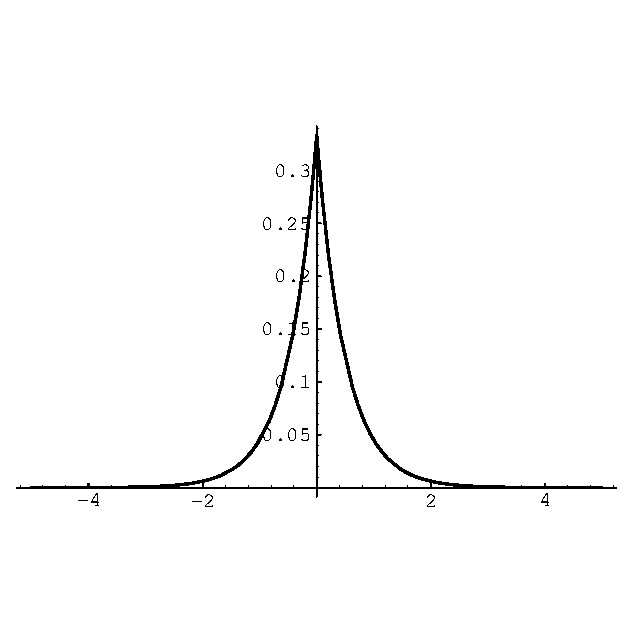
\includegraphics[width=0.4\textwidth]{ode/inhomogeneous/wrongsol}
    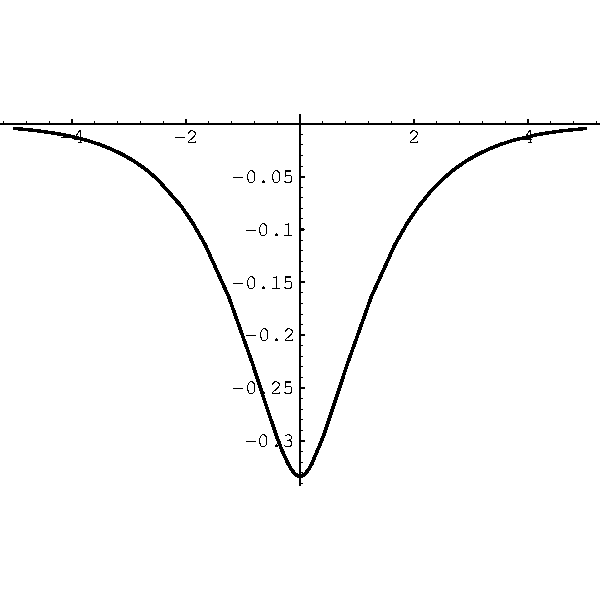
\includegraphics[width=0.4\textwidth]{ode/inhomogeneous/rightsol}
  \end{center}
  \caption{The incorrect and correct solution to the differential equation.}
  \label{wrong_right_sol}
\end{figure}







\begin{Example}
  Again consider
  \[ 
  y'' - y = \e^{-\alpha |x|}, \qquad y(\pm \infty) = 0, \qquad \alpha > 0, \alpha \neq 1. 
  \]
  Separating this into two problems for positive and negative $x$,
  \begin{alignat*}{3}
    y_-'' - y_- &= \e^{\alpha x}, &\quad &y_-(-\infty) = 0, &\quad &\mathrm{on}\ -\infty < x \leq 0, \\
    y_+'' - y_+ &= \e^{-\alpha x}, &\quad &y_+(\infty)=0, &\quad &\mathrm{on}\ 0\leq x < \infty.
  \end{alignat*}
  In order for the solution over the whole domain to be twice
  differentiable, the solution and its first derivative must be
  continuous.  Thus we impose the additional boundary conditions
  \[ 
  y_-(0) = y_+(0), \qquad y_-'(0) = y_+'(0). 
  \]
  The solutions that satisfy the two differential equations and the 
  boundary conditions at infinity are
  \[ 
  y_- = \frac{\e^{\alpha x}}{\alpha^2-1} + c_- \e^x, \qquad
  y_+ = \frac{\e^{-\alpha x}}{\alpha^2-1} + c_+ \e^{-x}. 
  \]
  The two additional boundary conditions give us the equations
  \begin{alignat*}{3}
    y_-(0) &= y_+(0) &\quad &\to &\quad &c_- = c_+ \\
    y_-'(0) &= y_+'(0) &\quad &\to &\quad &\frac{\alpha}{\alpha^2-1} + c_- = 
    -\frac{\alpha}{\alpha^2-1} - c_+.
  \end{alignat*}
  We solve these two equations to determine $c_-$ and $c_+$.
  \[ 
  c_- = c_+ = - \frac{\alpha}{\alpha^2-1}
  \]
  Thus the solution over the whole domain is
  \[ 
  y =  \begin{cases}
    \frac{\e^{\alpha x} - \alpha \e^x }{\alpha^2-1} &\mathrm{for}\ x < 0, \\
    \frac{\e^{-\alpha x}-\alpha \e^{-x}}{\alpha^2-1} &\mathrm{for}\ x > 0
  \end{cases}
  \]
  \[ 
  \boxed{ 
    y = \frac{\e^{-\alpha |x|} - \alpha \e^{-|x|}}{\alpha^2-1}. 
    }
  \]
  This function is plotted in Figure~\ref{wrong_right_sol}.
  You can verify that this solution is twice continuously differentiable.
\end{Example}














%%=============================================================================
\section{Inhomogeneous Boundary Conditions}



%%-----------------------------------------------------------------------------
\subsection{Eliminating Inhomogeneous Boundary Conditions}


Consider the $n^{t h}$ order equation
\[
L[y] = f(x), \quad \mathrm{for}\ a < x < b,
\]
subject to the linear inhomogeneous boundary conditions
\[ B_j[y] = \gamma_j, \quad \mathrm{for}\ j = 1, \ldots, n, \]
where the boundary conditions are of the form
\[
B[y] \equiv \alpha_0 y(a) + \alpha_1 y'(a) + \cdots + y_{n-1} y^{(n-1)}(a)
+ \beta_0 y(b) + \beta_1 y'(b) + \cdots + \beta_{n-1} y^{(n-1)}
\]
Let $g(x)$ be an $n$-times continuously differentiable function that 
satisfies the boundary conditions.  Substituting $y = u + g$ into the 
differential equation and boundary conditions yields
\[ L[u] = f(x) - L[g], \qquad B_j[u] = b_j - B_j[g] = 0 
\quad \mathrm{for}\ j = 1,\ldots,n.\]
Note that the problem for $u$ has homogeneous boundary conditions.  Thus a
problem with inhomogeneous boundary conditions can be reduced to one with
homogeneous boundary conditions.  This technique is of limited usefulness
for ordinary differential equations but is important for solving some 
partial differential equation problems.






\begin{Example}
  Consider the problem
  \[ y'' + y = \cos 2x, \qquad y(0) = 1, \quad y(\pi) = 2.\]
  $g(x) = \frac{x}{\pi} + 1$ satisfies the boundary conditions.  Substituting
  $y = u + g$ yields
  \[ u'' + u = \cos 2x - \frac{x}{\pi} - 1, \qquad y(0) = y(\pi) = 0. \]
\end{Example}







\begin{Example}
  Consider
  \[ y'' + y = \cos 2x, \qquad y'(0) = y(\pi) = 1. \]
  $g(x) = \sin x - \cos x$ satisfies the inhomogeneous boundary conditions.
  Substituting $y = u + \sin x - \cos x$ yields
  \[ u'' + u = \cos 2x, \qquad u'(0) = u(\pi) = 0. \]
  Note that since $g(x)$ satisfies the homogeneous equation, the inhomogeneous
  term in the equation for $u$ is the same as that in the equation for $y$.
\end{Example}









\begin{Example}
  Consider
  \[ y'' + y = \cos 2x, \qquad y(0) = \frac{2}{3}, \quad y(\pi) = -\frac{4}{3}. \]
  $g(x) = \cos x - \frac{1}{3}$ satisfies the boundary conditions.  Substituting
  $y = u + \cos x - \frac{1}{3}$ yields
  \[ u'' + u = \cos 2x + \frac{1}{3}, \qquad u(0) = u(\pi) = 0. \]
\end{Example}











\begin{Result}
  The $n^{th}$ order differential equation with boundary conditions
  \[
  L[y]=f(x), \qquad B_j[y]=b_j, \quad \mathrm{for}\ j = 1,\ldots,n
  \]
  has the solution $y = u + g$ where $u$ satisfies
  \[
  L[u] = f(x) - L[g], \qquad B_j[u] = 0, \quad \mathrm{for}\ j= 1, \ldots, n
  \]
  and $g$ is any $n$-times continuously differentiable function that satisfies
  the inhomogeneous boundary conditions.
\end{Result}










%%-----------------------------------------------------------------------------
\subsection{Separating Inhomogeneous Equations and Inhomogeneous Boundary 
  Conditions}

Now consider a problem with inhomogeneous boundary conditions
\[ L[y] = f(x), \quad B_1[y] = \gamma_1, \quad B_2[y] = \gamma_2.\]
In order to solve this problem, we solve the two problems
\[ L[u] = f(x), \quad B_1[u] = B_2[u] = 0, \quad \mathrm{and}\]
\[ L[v] = 0, \quad B_1[v] = \gamma_1, \quad B_2[v] = \gamma_2.\]
The solution for the problem with an inhomogeneous equation and
inhomogeneous boundary conditions will be the sum of $u$ and $v$.
To verify this,
\begin{gather*}
  L[u+v] = L[u] + L[v] = f(x) + 0 = f(x), \\
  B_i[u + v] = B_i[u] + B_i[v] = 0 + \gamma_i = \gamma_i.
\end{gather*}
This will be a useful technique when we develop Green functions.


\begin{Result}
  The solution to
  \[ L[y] = f(x), \quad B_1[y] = \gamma_1, \quad B_2[y] = \gamma_2,\]
  is $y = u + v$ where
  \begin{alignat*}{3}
    L[u] &= f(x), &\quad B_1[u] &= 0, &\quad B_2[u] &= 0, \quad \mathrm{and} \\
    L[v] &= 0, &\quad B_1[v] &= \gamma_1, &\quad B_2[v] &= \gamma_2.
  \end{alignat*}
\end{Result}











%%-----------------------------------------------------------------------------
\subsection{Existence of Solutions of Problems with Inhomogeneous Boundary
  Conditions}

Consider the $n^{th}$ order homogeneous differential equation
\[
L[y] = y^{(n)} + p_{n-1} y^{(n-1)} + \cdots + p_1 y' + p_0 y = f(x), \quad
\mathrm{for}\ a < x < b,
\]
subject to the $n$ inhomogeneous boundary conditions
\[
B_j[y] = \gamma_j, \quad \mathrm{for}\ j = 1,\ldots,n
\]
where each boundary condition is of the form
\[
B[y] \equiv \alpha_0 y(a) + \alpha_1 y'(a) + \cdots + \alpha_{n-1} y^{(n-1)}(a)
+ \beta_0 y(b) + \beta_1 y'(b) + \cdots + \beta_{n-1} y^{(n-1)}(b).
\]
We assume that the coefficients in the differential equation are continuous
on $[a,b]$.  Since the Wronskian of the solutions of the differential 
equation,
\[
W(x) = \exp \left( - \int p_{n-1}(x) \,\dd x \right),
\]
is non-vanishing on $[a,b]$, there are $n$ linearly independent solution
on that range.   Let $\{y_1,\ldots,y_n\}$ be a set of linearly independent
solutions of the homogeneous equation.  From Result~\ref{ionvop} we know that
a particular solution $y_p$ exists.
The general solution of the differential equation is
\[
y = y_p + c_1 y_1 + c_2 y_2 + \cdots + c_n y_n.
\]
The $n$ boundary conditions impose the matrix equation,
\[
\begin{pmatrix}
  B_1[y_1] & B_1[y_2] & \cdots & B_1[y_n] \\
  B_2[y_1] & B_2[y_2] & \cdots & B_2[y_n] \\
  \vdots   & \vdots   & \ddots & \vdots   \\
  B_n[y_1] & B_n[y_2] & \cdots & B_n[y_n] 
\end{pmatrix}
\ 
\begin{pmatrix}
  c_1 \\
  c_2 \\
  \vdots \\
  c_n
\end{pmatrix}
=
\begin{pmatrix}
  \gamma_1 - B_1[y_p] \\
  \gamma_2 - B_2[y_p] \\
  \vdots \\
  \gamma_n - B_n[y_p]
\end{pmatrix}
\]
This equation has a unique solution if and only if the equation
\[
\begin{pmatrix}
  B_1[y_1] & B_1[y_2] & \cdots & B_1[y_n] \\
  B_2[y_1] & B_2[y_2] & \cdots & B_2[y_n] \\
  \vdots   & \vdots   & \ddots & \vdots   \\
  B_n[y_1] & B_n[y_2] & \cdots & B_n[y_n] 
\end{pmatrix}
\ 
\begin{pmatrix}
  c_1 \\
  c_2 \\
  \vdots \\
  c_n
\end{pmatrix}
=
\begin{pmatrix}
  0 \\
  0 \\
  \vdots \\
  0 \\
\end{pmatrix}
\]
has only the trivial solution.  (This is the case if and only if the 
determinant of the matrix is nonzero.)
Thus the problem
\[
L[y] = y^{(n)} + p_{n-1} y^{(n-1)} + \cdots + p_1 y' + p_0 y = f(x), \quad
\mathrm{for}\ a < x < b,
\]
subject to the $n$ inhomogeneous boundary conditions
\[
B_j[y] = \gamma_j, \quad \mathrm{for}\ j = 1,\ldots,n,
\]
has a unique solution if and only if the problem
\[
L[y] = y^{(n)} + p_{n-1} y^{(n-1)} + \cdots + p_1 y' + p_0 y = 0, \quad
\mathrm{for}\ a < x < b,
\]
subject to the $n$ homogeneous boundary conditions
\[
B_j[y] = 0, \quad \mathrm{for}\ j = 1,\ldots,n,
\]
has only the trivial solution.








\begin{Result}
  \label{ioeostie}
  The problem
  \[
  L[y] = y^{(n)} + p_{n-1} y^{(n-1)} + \cdots + p_1 y' + p_0 y = f(x), \quad
  \mathrm{for}\ a < x < b,
  \]
  subject to the $n$ inhomogeneous boundary conditions
  \[
  B_j[y] = \gamma_j, \quad \mathrm{for}\ j = 1,\ldots,n,
  \]
  has a unique solution if and only if the problem
  \[
  L[y] = y^{(n)} + p_{n-1} y^{(n-1)} + \cdots + p_1 y' + p_0 y = 0, \quad
  \mathrm{for}\ a < x < b,
  \]
  subject to 
  \[
  B_j[y] = 0, \quad \mathrm{for}\ j = 1,\ldots,n,
  \]
  has only the trivial solution.
\end{Result}








%%============================================================================
\section{Green Functions for First Order Equations}



Consider the first order inhomogeneous equation
\begin{equation}
  \label{eqn y'+py=f}
  L[y] \equiv y' + p(x) y = f(x), \quad \mathrm{for}\ x > a,
\end{equation}
subject to a homogeneous initial condition, $B[y] \equiv y(a) = 0$.

The Green function $G(x|\xi)$ is defined as the solution to
\[ 
L[G(x|\xi)] = \delta(x-\xi) \quad \mathrm{subject to}\ G(a|\xi) = 0.
\]
We can represent the 
solution to the inhomogeneous problem in Equation~\ref{eqn y'+py=f}
as an integral involving the Green function.  To show that
\[
y(x) = \int_a^\infty G(x|\xi) f(\xi)\,\dd \xi
\]
is the solution, we apply the linear operator $L$ to the integral.
(Assume that the integral is uniformly convergent.)
\begin{align*}
  L\left[ \int_a^\infty G(x|\xi) f(\xi)\,\dd \xi\right] 
  &= \int_a^\infty L[G(x|\xi)] f(\xi)\,\dd \xi 
  \\
  &= \int_a^\infty \delta(x-\xi) f(\xi)\,\dd \xi 
  \\
  &= f(x)
\end{align*}
The integral also satisfies the initial condition.
\begin{align*}
  B\left[ \int_a^\infty G(x|\xi) f(\xi)\,\dd \xi\right]
  &= \int_a^\infty B[G(x|\xi)] f(\xi)\,\dd \xi 
  \\
  &= \int_a^\infty (0) f(\xi)\,\dd \xi 
  \\
  &= 0
\end{align*}

Now we consider the qualitiative behavior of the Green function.  For 
$x \neq \xi$, the Green function is simply a homogeneous solution of the 
differential equation, however at $x = \xi$ we expect some singular behavior.
$G'(x|\xi)$ will have a Dirac delta function type singularity.  This means that
$G(x|\xi)$ will have a jump discontinuity at $x = \xi$.
We integrate the differential equation on the vanishing interval 
$(\xi^- \ldots \xi^+)$ to determine this jump.
\begin{gather}
  G' + p(x) G = \delta(x-\xi)
  \nonumber
  \\
  G(\xi^+|\xi) - G(\xi^-|\xi) + \int_{\xi^-}^{\xi^+} p(x) G(x|\xi) \,\dd x = 1
  \nonumber
  \\
  \label{eqn first order G+ - G- = 1}
  G(\xi^+|\xi) - G(\xi^-|\xi) = 1
\end{gather}

The homogeneous solution of the differential equation is
\[
y_h = \e^{-\int p(x) \,\dd x}
\]
Since the Green function satisfies the 
homogeneous equation for $x \neq \xi$, it will be a constant times this
homogeneous solution for $x < \xi$ and $x > \xi$.
\[
G(x|\xi) = 
\begin{cases}
  c_1 \e^{-\int p(x) \,\dd x} \quad &a < x < \xi \\
  c_2 \e^{-\int p(x) \,\dd x} \quad &\xi < x
\end{cases}
\]
In order to satisfy the homogeneous initial condition $G(a|\xi) = 0$, the 
Green function must vanish on the interval $(a \ldots \xi)$.
\[
G(x|\xi) = 
\begin{cases}
  0 \quad &a < x < \xi \\
  c \e^{-\int p(x) \,\dd x} \quad &\xi < x
\end{cases}
\]
The jump condition, (Equation~\ref{eqn first order G+ - G- = 1}), 
gives us the constraint $G(\xi^+|\xi) = 1$.  This determines the constant in 
the homogeneous solution for $x > \xi$.
\[
G(x|\xi) = 
\begin{cases}
  0 \quad &a < x < \xi \\
  \e^{-\int_\xi^x p(t) \,\dd t} \quad &\xi < x
\end{cases}
\]
We can use the Heaviside function to write the Green function without using 
a case statement.
\[
G(x|\xi) = \e^{-\int_\xi^x p(t) \,\dd t} H(x-\xi)
\]


Clearly the Green function is of little value in solving the inhomogeneous
differential equation in Equation~\ref{eqn y'+py=f}, as we can solve that
problem directly.  However, we will encounter first order Green function
problems in solving some partial differential equations.



\begin{Result}
  The first order inhomogeneous differential equation with homogeneous 
  initial condition
  \[ 
  L[y] \equiv y' + p(x) y = f(x), \quad \mathrm{for}\ a < x,
  \qquad y(a) = 0,
  \]
  has the solution
  \[ 
  y = \int_a^\infty G(x|\xi)f(\xi)\,\dd \xi,
  \]
  where $G(x|\xi)$ satisfies the equation
  \[ 
  L[G(x|\xi)] = \delta(x-\xi), \quad \mathrm{for}\ a<x, \qquad
  G(a|\xi) = 0.
  \]
  The Green function is
  \[
  G(x|\xi) = \e^{-\int_\xi^x p(t) \,\dd t} H(x-\xi)
  \]
\end{Result}














%%============================================================================
\section{Green Functions for Second Order Equations}


Consider the second order inhomogeneous equation
\begin{equation}
  \label{eqn y''+py'+qy=f}
  L[y] = y'' + p(x) y' + q(x) y = f(x), \quad \mathrm{for}\ a < x < b,
\end{equation}
subject to the homogeneous boundary conditions
\[ 
B_1[y] = B_2[y] = 0.
\]

The Green function $G(x|\xi)$ is defined as the solution to
\[ 
L[G(x|\xi)] = \delta(x-\xi) \quad \mathrm{subject to}\ B_1[G]=B_2[G]=0.
\]
The Green function is useful because you can represent the 
solution to the inhomogeneous problem in Equation~\ref{eqn y''+py'+qy=f}
as an integral involving the Green function.  To show that
\[
y(x) = \int_a^b G(x|\xi) f(\xi)\,\dd \xi
\]
is the solution, we apply the linear operator $L$ to the integral.
(Assume that the integral is uniformly convergent.)
\begin{align*}
  L\left[ \int_a^b G(x|\xi) f(\xi)\,\dd \xi\right] 
  &= \int_a^b L[G(x|\xi)] f(\xi)\,\dd \xi 
  \\
  &= \int_a^b \delta(x-\xi) f(\xi)\,\dd \xi 
  \\
  &= f(x)
\end{align*}
The integral also satisfies the boundary conditions.
\begin{align*}
  B_i\left[ \int_a^b G(x|\xi) f(\xi)\,\dd \xi\right]
  &= \int_a^b B_i[G(x|\xi)] f(\xi)\,\dd \xi 
  \\
  &= \int_a^b [0] f(\xi)\,\dd \xi 
  \\
  &= 0
\end{align*}

One of the advantages of using Green functions is that once you find 
the Green function for a linear operator and certain homogeneous boundary 
conditions, 
\[
L[G] = \delta(x-\xi), \quad B_1[G] = B_2[G] = 0,
\]
you can write the solution
for any inhomogeneity, $f(x)$.  
\[
L[f] = f(x), \quad B_1[y] = B_2[y] = 0
\]
You do not need to do any extra work to 
obtain the solution for a different inhomogeneous term.

Qualitatively, what kind of behavior will the Green function for 
a second order differential equation have?  Will it have a delta function
singularity; will it be continuous?  To answer these questions
we will first look at the behavior of integrals and derivatives of $\delta(x)$.

The integral of $\delta(x)$ is the Heaviside function, $H(x)$.
\[
H(x) = \int_{-\infty}^x \delta(t)\,\dd t = 
\begin{cases}
  0 \quad &\mathrm{for}\ x < 0 \\
  1 \quad &\mathrm{for}\ x > 0
\end{cases}
\]
The integral of the Heaviside function is the ramp function, $r(x)$.
\[ 
r(x) = \int_{-\infty}^x H(t)\,\dd t = 
\begin{cases}
  0 \quad &\mathrm{for}\ x < 0 \\
  x \quad &\mathrm{for}\ x > 0
\end{cases}
\]
The derivative of the delta function is zero for $x \neq 0$.  At $x=0$
it goes from $0$ up to $+\infty$, down to $-\infty$ and then back
up to $0$.

In Figure~\ref{fig_delta} we see conceptually the behavior of the ramp 
function, the Heaviside function, the delta function, and the derivative of the
delta function.






\begin{figure}[tb!]
  \begin{center} 
    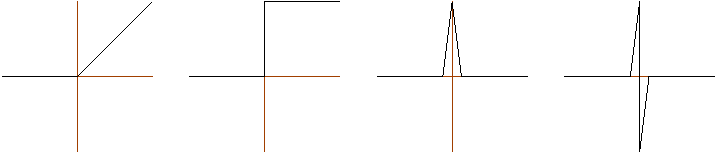
\includegraphics[width=\textwidth]{ode/inhomogeneous/delta}
  \end{center}
  \caption{The ramp function, the Heaviside function, the delta function, 
    and the derivative of the delta function.}
  \label{fig_delta}
\end{figure}



We write the differential equation for the Green function.
\[
G''(x|\xi) + p(x) G'(x|\xi) + q(x) G(x|\xi) = \delta(x-\xi)
\]
we see that only the $G''(x|\xi)$ term can have a delta function type 
singularity.  If one of the other terms had a delta function type singularity
then $G''(x|\xi)$ would be more singular than a delta function and there
would be nothing in the right hand side of the equation to match this 
kind of singularity.  
Analogous to the progression from a delta function to a Heaviside function
to a ramp function,
we see that $G'(x|\xi)$ will have a jump discontinuity and $G(x|\xi)$ will
be continuous.

Let $y_1$ and $y_2$ be two linearly independent solutions to the homogeneous
equation, $L[y] = 0$.  Since the Green function satisfies the 
homogeneous equation for $x \neq \xi$, it will be a linear combination of
the homogeneous solutions.
\[
G(x|\xi) = 
\begin{cases}
  c_1 y_1 + c_2 y_2 \quad &\mathrm{for}\ x < \xi \\
  d_1 y_1 + d_2 y_2 \quad &\mathrm{for}\ x > \xi
\end{cases}
\]

We require that $G(x|\xi)$ be continuous.
\begin{gather*}
  G(x|\xi)\big|_{x \to \xi^-} = G(x|\xi)\big|_{x \to \xi^+} 
  \\
  \intertext{We can write this in terms of the homogeneous solutions.}
  c_1 y_1(\xi) + c_2 y_2(\xi) = d_1 y_1(\xi) + d_2 y_2(\xi)
\end{gather*}

We integrate $L[G(x|\xi)] = \delta(x-\xi)$ from $\xi^-$ to $\xi+$.
\begin{gather*}
  \int_{\xi^-}^{\xi^+} \left[G''(x|\xi) + p(x)G'(x|\xi)+q(x)G(x|\xi) \right]\,\dd x = 
  \int_{\xi^-}^{\xi^+} \delta(x-\xi)\,\dd x. 
  \\
  \intertext{Since $G(x|\xi)$ is continuous and $G'(x|\xi)$ has only a 
    jump discontinuity two of the terms vanish.}
  \int_{\xi^-}^{\xi^+} p(x) G'(x|\xi)\,\dd x = 0 \qquad \mathrm{and} \qquad
  \int_{\xi^-}^{\xi^+} q(x) G(x|\xi)\,\dd x = 0
  \\
  \int_{\xi^-}^{\xi^+} G''(x|\xi)\,\dd x = \int_{\xi^-}^{\xi^+} \delta(x-\xi)\,\dd x 
  \\
  \big[ G'(x|\xi) \big]_{\xi^-}^{\xi^+}
  = \big[ H(x-\xi) \big]_{\xi^-}^{\xi^+} 
  \\
  G'(\xi^+|\xi) - G'(\xi^-|\xi) = 1
  \\
  \intertext{We write this jump condition in terms of the homogeneous 
    solutions.}
  d_1 y_1'(\xi) + d_2 y_2'(\xi) - c_1 y_1'(\xi) - c_2 y_2'(\xi) = 1
\end{gather*}
Combined with the two boundary conditions, this gives us a total of 
four equations to determine our four constants, $c_1$, $c_2$, $d_1$, and $d_2$.




\begin{Result}
  The second order inhomogeneous differential equation with homogeneous 
  boundary conditions
  \[ 
  L[y] = y'' + p(x)y' + q(x) y = f(x), \quad \mathrm{for}\ a < x < b, 
  \qquad B_1[y] = B_2[y] = 0,
  \]
  has the solution
  \[ 
  y = \int_a^b G(x|\xi)f(\xi)\,\dd \xi,
  \]
  where $G(x|\xi)$ satisfies the equation
  \[ 
  L[G(x|\xi)] = \delta(x-\xi), \quad \mathrm{for}\ a<x<b, \qquad
  B_1[G(x|\xi)] = B_2[G(x|\xi)] = 0.
  \]
  $G(x|\xi)$ is continuous and $G'(x|\xi)$ has a jump discontinuity of
  height $1$ at $x = \xi$.
\end{Result}






\begin{Example} \label{greens_fx}
  Solve the boundary value problem
  \[y'' = f(x), \qquad y(0) = y(1) = 0,\]
  using a Green function.

  A pair of solutions to the homogeneous equation are $y_1 = 1$ and $y_2 = x$.
  First note that only the trivial solution to the homogeneous equation
  satisfies the homogeneous boundary conditions.  Thus there is a unique solution
  to this problem.

  The Green function satisfies 
  \[ G''(x|\xi) = \delta(x-\xi), \qquad G(0|\xi) = G(1|\xi) = 0.\]
  The Green function has the form
  \[ G(x|\xi) = 
  \begin{cases}
    c_1 + c_2 x \quad &\mathrm{for}\ x < \xi \\
    d_1 + d_2 x \quad &\mathrm{for}\  x > \xi.
  \end{cases}
  \]
  Applying the two boundary conditions, we see that $c_1 = 0$ and $d_1=-d_2$.
  The Green function now has the form
  \[ G(x|\xi) = 
  \begin{cases}
    c x \quad &\mathrm{for}\  x < \xi \\
    d(x-1) \quad &\mathrm{for}\  x > \xi.
  \end{cases}
  \]
  Since the Green function must be continuous,
  \[ c \xi = d(\xi-1) \quad \to \quad d = c \frac{\xi}{\xi-1}.\]
  From the jump condition,
  \begin{gather*}
    \frac{\dd}{\dd x} c \frac{\xi}{\xi-1} (x-1) \Big|_{x=\xi} 
    - \frac{\dd}{\dd x} c x \Big|_{x=\xi} = 1 \\
    c \frac{\xi}{\xi-1} - c = 1 \\
    c = \xi-1.
  \end{gather*}
  Thus the Green function is
  \[ \boxed{ G(x|\xi) = 
    \begin{cases}
      (\xi-1) x \quad &\mathrm{for}\ x < \xi \\
      \xi(x-1) \quad &\mathrm{for}\ x > \xi.
    \end{cases} }
  \]
  The Green function is plotted in Figure~\ref{greens_x} for various values
  of $\xi$.  We show $G(x|0.05)$, $G(x|0.25)$, $G(x|0.5)$ and $G(x|0.75)$.
  The solution to $y'' = f(x)$ is

  \[ y(x) = \int_0^1 G(x|\xi) f(\xi)\,\dd \xi \]
  \[ \boxed{ y(x) = (x-1) \int_0^x \xi f(\xi)\,\dd \xi 
    + x \int_x^1 (\xi - 1) f(\xi)\,\dd \xi. } \]

  \begin{figure}[tb!]
    \begin{center}
      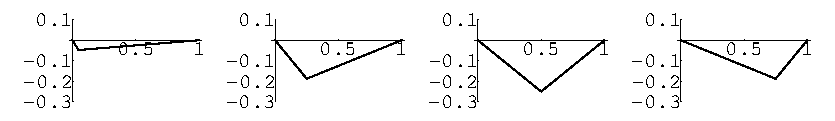
\includegraphics[width=\textwidth]{ode/inhomogeneous/greensx}
    \end{center}
    \caption{Plots of the Green functions.} 
    \label{greens_x}
  \end{figure}

\end{Example}














\begin{Example}
  Solve the boundary value problem
  \[ 
  y'' = f(x), \qquad y(0) = 1, \quad y(1) = 2.
  \]

  In Example~\ref{greens_fx} we saw that the solution to
  \[ 
  u'' = f(x), \qquad u(0) = u(1) = 0 
  \]
  is
  \[ 
  u(x) = (x-1) \int_0^x \xi f(\xi)\,\dd \xi + x \int_x^1 (\xi - 1) f(\xi)\,\dd \xi.
  \]

  Now we have to find the solution to
  \[ 
  v'' = 0, \qquad v(0) = 1, \quad u(1) = 2.
  \]
  The general solution is
  \[ 
  v = c_1 + c_2 x.
  \]
  Applying the boundary conditions yields
  \[ 
  v = 1 + x.
  \]

  Thus the solution for $y$ is
  \[ 
  \boxed{
    y = 1 + x + (x-1) \int_0^x \xi f(\xi)\,\dd \xi 
    + x \int_x^1 (\xi - 1) f(\ xi)\,\dd \xi.
    }
  \]
\end{Example}

















\begin{Example}
  Consider
  \[ 
  y'' = x, \qquad y(0) = y(1) = 0. 
  \]

  \paragraph{Method 1.}
  Integrating the differential equation twice yields
  \[ 
  y = \frac{1}{6} x^3 + c_1 x + c_2. 
  \]
  Applying the boundary conditions, we find that the solution is
  \[ 
  \boxed{ 
    y = \frac{1}{6} (x^3 - x). 
    } 
  \]

  \paragraph{Method 2.}
  Using the Green function to find the solution,
  \begin{align*}
    y       &= (x-1) \int_0^x \xi^2 \,\dd \xi + x \int_x^1 (\xi-1)\xi\,\dd \xi \\
    &= (x-1) \frac{1}{3} x^3 + x \left( \frac{1}{3} - \frac{1}{2}
      -\frac{1}{3} x^3 + \frac{1}{2} x^2 \right)
  \end{align*}
  \[ 
  \boxed{ 
    y = \frac{1}{6} (x^3 - x). 
    } 
  \]
\end{Example}














\begin{Example} \label{greens_sinx}
  Find the solution to the differential equation
  \[ 
  y'' - y = \sin x, 
  \]
  that is bounded for all $x$.

  The Green function for this problem satisfies
  \[
  G''(x|\xi) - G(x|\xi) = \delta(x-\xi).
  \]
  The homogeneous solutions are $y_1 = \e^x$, and $y_2 = \e^{-x}$.
  The Green function has the form
  \[ 
  G(x|\xi) = 
  \begin{cases}
    c_1 \e^x + c_2 \e^{-x} \quad &\mathrm{for}\ x < \xi \\
    d_1 \e^x + d_2 \e^{-x} \quad &\mathrm{for}\ x > \xi. 
  \end{cases}
  \]
  Since the solution must be bounded for all $x$, the Green function must
  also be bounded.  Thus $c_2 = d_1 = 0$.  
  The Green function now has the form
  \[ 
  G(x|\xi) = 
  \begin{cases}
    c \e^x \quad &\mathrm{for}\ x < \xi \\
    d \e^{-x} \quad &\mathrm{for}\ x > \xi. 
  \end{cases}
  \]
  Requiring that $G(x|\xi)$ be continuous gives us the condition
  \[ 
  c \e^\xi = d \e^{-\xi} \quad \to \quad d = c \e^{2\xi}.
  \]
  $G(x|\xi)$ has a jump discontinuity of height $1$ at $x = \xi$.
  \begin{gather*}
    \frac{\dd}{\dd x}c \e^{2\xi} \e^{-x}\bigg|_{x=\xi} 
    - \frac{\dd}{\dd x} c \e^x\bigg|_{x=\xi} = 1 \\
    -c \e^{2\xi} \e^{-\xi} - c \e^\xi = 1 \\
    c = -\frac{1}{2} \e^{-\xi}
  \end{gather*}
  The Green function is then
  \[ 
  G(x|\xi) = 
  \begin{cases}
    -\frac{1}{2} \e^{x-\xi} \quad &\mathrm{for}\ x < \xi \\
    -\frac{1}{2} \e^{-x+\xi} \quad &\mathrm{for}\ x > \xi 
  \end{cases} 
  \]
  \[ 
  \boxed{ 
    G(x|\xi) = -\frac{1}{2} \e^{-|x-\xi|}. 
    } 
  \]
  A plot of $G(x|0)$ is given in Figure~\ref{greens_ex}. 
  The solution to $y'' - y = \sin x$ is
  \begin{align*}
    y(x) &= \int_{-\infty}^\infty -\frac{1}{2} \e^{-|x-\xi|} \sin\xi\,\dd \xi \\
    &= -\frac{1}{2} \left( \int_{-\infty}^x \sin\xi \e^{x-\xi}\,\dd \xi + 
      \int_x^\infty \sin\xi \e^{-x+\xi}\,\dd \xi \right) \\
    &= -\frac{1}{2} (-\frac{\sin x+\cos x}{2} +\frac{-\sin x+\cos x}{2})
  \end{align*}
  \[ 
  \boxed{ 
    y = \frac{1}{2} \sin x. 
    } 
  \]
  \begin{figure}[tb!]
    \begin{center}
      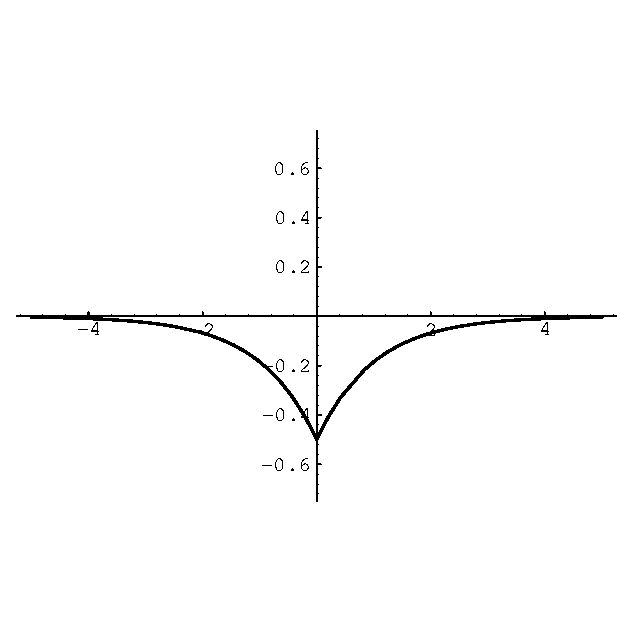
\includegraphics[width=0.5\textwidth]{ode/inhomogeneous/greens1}
    \end{center}
    \caption{Plot of the Green function.} 
    \label{greens_ex}
  \end{figure}

\end{Example}






%%-------------------------------------------------------------------------
\subsection{Green Functions for Sturm-Liouville Problems}



Consider the problem
\begin{gather*}
  L[y] = \left( p(x) y' \right)' + q(x) y = f(x), 
  \quad \mathrm{subject to}
  \\
  B_1[y] = \alpha_1 y(a) + \alpha_2 y'(a) = 0, \quad
  B_2[y] = \beta_1 y(b) + \beta_2 y'(b) = 0. 
\end{gather*}
This is known as a Sturm-Liouville problem.  Equations of this type
often occur when solving partial differential equations.
The Green function associated with this problem satisfies
\[ 
L[G(x|\xi)] = \delta(x-\xi), \quad B_1[G(x|\xi)] = B_2[G(x|\xi)] = 0.
\]
Let $y_1$ and $y_2$ be two non-trivial homogeneous solutions that satisfy
the left and right boundary conditions, respectively.
\[ 
L[y_1] = 0, \quad B_1[y_1] = 0, \qquad L[y_2] = 0, \quad B_2[y_2] = 0. 
\]
The Green function satisfies the homogeneous equation for $x \neq \xi$ 
and satisfies the homogeneous boundary conditions.
Thus it must have the following form.
\[ 
G(x|\xi) = 
\begin{cases}
  c_1(\xi) y_1(x) \quad &\mathrm{for}\ a \leq x \leq \xi, \\
  c_2(\xi) y_2(x) \quad &\mathrm{for}\ \xi \leq x \leq b,
\end{cases}
\]
Here $c_1$ and $c_2$ are unknown functions of $\xi$.

The first constraint on $c_1$ and $c_2$ comes from the continuity condition.
\begin{gather*}
  G(\xi^-|\xi) = G(\xi^+|\xi)
  \\
  c_1(\xi) y_1(\xi) = c_2(\xi) y_2(\xi)
\end{gather*}
We write the inhomogeneous equation in the standard form.
\[ 
G''(x|\xi) + \frac{p'}{p} G'(x|\xi) + \frac{q}{p} G(x|\xi) = \frac{\delta(x-\xi)}{p}
\]
The second constraint on $c_1$ and $c_2$ comes from the jump condition.
\begin{gather*}
  G'(\xi^+|\xi) -  G'(\xi^-|\xi) = \frac{1}{p(\xi)} 
  \\
  c_2(\xi) y_2'(\xi) - c_1(\xi) y_1'(\xi) = \frac{1}{p(\xi)}
\end{gather*}
Now we have a system of equations to determine $c_1$ and $c_2$.
\begin{align*}
  c_1(\xi) y_1(\xi) - c_2(\xi) y_2(\xi) &= 0 
  \\
  c_1(\xi) y_1'(\xi) - c_2(\xi) y_2'(\xi) &= -\frac{1}{p(\xi)}
\end{align*}
We solve this system with Kramer's rule.
\[ 
c_1(\xi) = -\frac{y_2(\xi)}{p(\xi) (-W(\xi))}, \quad
c_2(\xi) = - \frac{y_1(\xi)}{p(\xi) (-W(\xi))}
\]
Here $W(x)$ is the Wronskian of $y_1(x)$ and $y_2(x)$.  
The Green function is
\[ 
\boxed{ 
  G(x|\xi) = 
  \begin{cases}
    \frac{y_1(x) y_2(\xi)}{p(\xi) W(\xi)} \quad &\mathrm{for}\ a \leq x \leq \xi, 
    \\
    \frac{y_2(x) y_1(\xi)}{p(\xi) W(\xi)} \quad &\mathrm{for}\ \xi \leq x \leq b.
  \end{cases} 
  }
\]
The solution of the Sturm-Liouville problem is 
\[
y = \int_a^b G(x|\xi) f(\xi) \,\dd \xi.
\]



\begin{Result}
  The problem
  \begin{gather*}
    L[y] = \left( p(x) y' \right)' + q(x) y = f(x), 
    \quad \mathrm{subject to}
    \\
    B_1[y] = \alpha_1 y(a) + \alpha_2 y'(a) = 0, \quad
    B_2[y] = \beta_1 y(b) + \beta_2 y'(b) = 0. 
  \end{gather*}
  has the Green function
  \[ 
  G(x|\xi) = 
  \begin{cases}
    \frac{y_1(x) y_2(\xi)}{p(\xi) W(\xi)} \quad &\mathrm{for}\ a \leq x \leq \xi, 
    \\
    \frac{y_2(x) y_1(\xi)}{p(\xi) W(\xi)} \quad &\mathrm{for}\ \xi \leq x \leq b,
  \end{cases} 
  \]
  where $y_1$ and $y_2$ are non-trivial homogeneous solutions that satisfy
  $B_1[y_1] = B_2[y_2] = 0$, and $W(x)$ is the Wronskian of $y_1$ and $y_2$.
\end{Result}








\begin{Example}
  Consider the equation
  \[ 
  y'' - y = f(x), \qquad y(0) = y(1) = 0.
  \]
  A set of solutions to the homogeneous equation is $\{ \e^x, \e^{-x} \}$.  
  Equivalently, one could use the set $\{ \cosh x, \sinh x \}$.
  Note that $\sinh x$ satisfies the left boundary condition and $\sinh (x-1)$
  satisfies the right boundary condition.
  The Wronskian of these two homogeneous solutions is
  \begin{align*}
    W(x)    
    &= \begin{vmatrix}
      \sinh x         &       \sinh (x-1)     \\
      \cosh x         &       \cosh(x-1)
    \end{vmatrix} 
    \\
    &= \sinh x \cosh(x-1) - \cosh x \sinh(x-1) 
    \\
    &= \frac{1}{2} [\sinh (2x-1) + \sinh (1) ]
    - \frac{1}{2} [\sinh (2x-1) - \sinh(1)] 
    \\
    &= \sinh (1).
  \end{align*}
  The Green function for the problem is then
  \[ 
  \boxed{ 
    G(x|\xi) = 
    \begin{cases}
      \frac{\sinh x \sinh(\xi-1)}{\sinh(1)} \quad &\mathrm{for}\ 0 \leq x \leq \xi \\
      \frac{\sinh(x-1) \sinh \xi}{\sinh(1)} \quad &\mathrm{for}\ \xi \leq x \leq 1.
    \end{cases} 
    } 
  \]
  The solution to the problem is
  \[ 
  \boxed{ 
    y = \frac{\sinh(x-1)}{\sinh(1)} \int_0^x \sinh(\xi) f(\xi)\,\dd \xi
    + \frac{\sinh(x)}{\sinh(1)} \int_x^1 \sinh(\xi-1) f(\xi)\,\dd \xi . 
    } 
  \]
\end{Example}




















%%-----------------------------------------------------------------------------
\subsection{Initial Value Problems}
Consider 
\[
L[y] = y'' + p(x) y' + q(x) y = f(x), \quad \mathrm{for}\ a < x < b,
\]
subject the the initial conditions
\[
y(a) = \gamma_1, \qquad y'(a) = \gamma_2.
\]
The solution is $y = u + v$ where
\[
u'' + p(x) u' + q(x) u = f(x), \qquad u(a) = 0, \quad u'(a) = 0,
\]
and
\[
v'' + p(x) v' + q(x) v = 0, \qquad v(a) = \gamma_1, \quad v'(a) = \gamma_2.
\]
Since the Wronskian
\[
W(x) = c \exp\left(-\int p(x)\,\dd x \right)
\]
is non-vanishing, the solutions of the differential equation for $v$ are 
linearly independent.  Thus there is a unique solution for $v$ that 
satisfies the initial conditions.

The Green function for $u$ satisfies
\[
G''(x|\xi) + p(x) G'(x|\xi) + q(x) G(x|\xi) = \delta(x-\xi), \qquad
G(a|\xi) = 0, \quad G'(a|\xi) = 0.
\]
The continuity and jump conditions are
\[
G(\xi^-|\xi) = G(\xi^+|\xi), \qquad G'(\xi^-|\xi) + 1 = G'(\xi^+|\xi).
\]
Let $u_1$ and $u_2$ be two linearly independent solutions of the 
differential equation.  For $x<\xi$, $G(x|\xi)$ is a linear combination 
of these solutions.  Since the Wronskian is non-vanishing, only the
trivial solution satisfies the homogeneous initial conditions.  The Green
function must be
\[
G(x|\xi) = 
\begin{cases}
  0 \quad &\mathrm{for}\ x < \xi \\
  u_\xi(x) \quad &\mathrm{for}\ x > \xi,
\end{cases}
\]
where $u_\xi(x)$ is the linear combination of $u_1$ and $u_2$ that satisfies
\[
u_\xi(\xi) = 0, \qquad u_\xi'(\xi) = 1.
\]
Note that the non-vanishing Wronskian ensures a unique solution for $u_\xi$.
We can write the Green function in the form
\[
G(x|\xi) = H(x-\xi) u_\xi(x).
\]
This is known as the \textbf{causal solution}.
The solution for $u$ is
\begin{align*}
  u       &= \int_a^b G(x|\xi) f(\xi) \,\dd \xi \\
  &= \int_a^b H(x-\xi) u_\xi(x) f(\xi) \,\dd \xi \\
  &= \int_a^x u_\xi(x) f(\xi) \,\dd \xi 
\end{align*}

Now we have the solution for $y$,
\[
y = v + \int_a^x u_\xi(x) f(\xi) \,\dd \xi.
\]



\begin{Result}
  The solution of the problem
  \[
  y'' + p(x) y' + q(x) y = f(x), \qquad y(a) = \gamma_1, \quad y'(a) = \gamma_2,
  \]
  is
  \[
  y = y_h + \int_a^x y_\xi(x) f(\xi) \,\dd \xi
  \]
  where $y_h$ is the combination of the homogeneous solutions of the equation 
  that satisfy the initial conditions and $y_\xi(x)$ is the linear combination
  of homogeneous solutions that satisfy $y_\xi(\xi) = 0$,
  $y_\xi'(\xi) = 1$.
\end{Result}










%%-----------------------------------------------------------------------------
\subsection{Problems with Unmixed Boundary Conditions}

Consider 
\[
L[y] = y'' + p(x) y' + q(x) y = f(x), \quad \mathrm{for}\ a < x < b,
\]
subject the the unmixed boundary conditions
\[
\alpha_1 y(a) + \alpha_2 y'(a) = \gamma_1, \qquad 
\beta_1 y(b) + \beta_2 y'(b) = \gamma_2.
\]
The solution is $y = u + v$ where
\[
u'' + p(x) u' + q(x) u = f(x), \qquad \alpha_1 u(a) + \alpha_2 u'(a) = 0, 
\quad \beta_1 u(b) + \beta_2 u'(b) = 0,
\]
and
\[
v'' + p(x) v' + q(x) v = 0, \qquad \alpha_1 v(a) + \alpha_2 v'(a) = \gamma_1, 
\quad \beta_1 v(b) + \beta_2 v'(b) = \gamma_2.
\]
The problem for $v$ may have no solution, a unique solution or an infinite
number of solutions.  We consider only the case that there is a unique solution
for $v$.  In this case the homogeneous equation subject to homogeneous
boundary conditions has only the trivial solution.

The Green function for $u$ satisfies
\[
G''(x|\xi) + p(x) G'(x|\xi) + q(x) G(x|\xi) = \delta(x-\xi), 
\]
\[
\alpha_1 G(a|\xi) + \alpha_2 G'(a|\xi) = 0, \quad 
\beta_1 G(b|\xi) + \beta_2 G'(b|\xi) = 0.
\]
The continuity and jump conditions are
\[
G(\xi^-|\xi) = G(\xi^+|\xi), \qquad G'(\xi^-|\xi) + 1 = G'(\xi^+|\xi).
\]
Let $u_1$ and $u_2$ be two solutions of the homogeneous equation that satisfy
the left and right boundary conditions, respectively.  The non-vanishing 
of the Wronskian ensures that these solutions exist.  Let $W(x)$ denote
the Wronskian of $u_1$ and $u_2$.  Since the homogeneous equation with 
homogeneous boundary conditions has only the trivial solution, $W(x)$ is
nonzero on $[a,b]$.  The Green function has the form
\[
G(x|\xi) = 
\begin{cases}
  c_1 u_1 \quad &\mathrm{for}\ x < \xi, \\
  c_2 u_2 \quad &\mathrm{for}\ x > \xi.
\end{cases}
\]
The continuity and jump conditions for Green function gives us the 
equations
\begin{align*}
  c_1 u_1(\xi) - c_2 u_2(\xi) &= 0 \\
  c_1 u_1'(\xi) - c_2 u_2'(\xi) &= -1.
\end{align*}
Using Kramer's rule, the solution is
\[
c_1 = \frac{u_2(\xi)}{W(\xi)}, \qquad
c_2 = \frac{u_1(\xi)}{W(\xi)}.
\]
Thus the Green function is
\[
G(x|\xi) = 
\begin{cases}
  \frac{u_1(x) u_2(\xi)}{W(\xi)} \quad &\mathrm{for}\ x < \xi, \\
  \frac{u_1(\xi) u_2(x)}{W(\xi)} \quad &\mathrm{for}\ x > \xi.
\end{cases}
\]
The solution for $u$ is
\[
u = \int_a^b G(x|\xi) f(\xi) \,\dd \xi.
\]
Thus if there is a unique solution for $v$, the solution for $y$ is
\[
y = v + \int_a^b G(x|\xi) f(\xi) \,\dd \xi.
\]




\begin{Result}
  Consider the problem
  \[
  y'' + p(x) y' + q(x) y = f(x), 
  \]
  \[
  \alpha_1 y(a) + \alpha_2 y'(a) = \gamma_1, \qquad
  \beta_1 y(b) + \beta_2 y'(b) = \gamma_2.
  \]
  If the homogeneous differential equation subject to the inhomogeneous 
  boundary conditions has the unique solution $y_h$, then the problem has 
  the unique solution
  \[
  y = y_h + \int_a^b G(x|\xi) f(\xi) \,\dd \xi
  \]
  where 
  \[
  G(x|\xi) =
  \begin{cases}
    \frac{u_1(x) u_2(\xi)}{W(\xi)} \quad &\mathrm{for}\ x < \xi, \\
    \frac{u_1(\xi) u_2(x)}{W(\xi)} \quad &\mathrm{for}\ x > \xi,
  \end{cases}
  \]
  $u_1$ and $u_2$ are solutions of the homogeneous differential equation that
  satisfy the left and right boundary conditions, respectively, and
  $W(x)$ is the Wronskian of $u_1$ and $u_2$.
\end{Result}











%%-----------------------------------------------------------------------------
\subsection{Problems with Mixed Boundary Conditions}

Consider 
\[
L[y] = y'' + p(x) y' + q(x) y = f(x), \quad \mathrm{for}\ a < x < b,
\]
subject the the mixed boundary conditions
\[
B_1[y] = \alpha_{11} y(a) + \alpha_{12} y'(a) 
+ \beta_{11} y(b) + \beta_{12} y'(b) = \gamma_1, 
\]
\[
B_2[y] = \alpha_{21} y(a) + \alpha_{22} y'(a) 
+ \beta_{21} y(b) + \beta_{22} y'(b) = \gamma_2. 
\]
The solution is $y = u + v$ where
\[
u'' + p(x) u' + q(x) u = f(x), \qquad B_1[u] = 0, 
\quad B_2[u] = 0,
\]
and
\[
v'' + p(x) v' + q(x) v = 0, \qquad B_1[v] = \gamma_1, 
\quad B_2[v] = \gamma_2.
\]

The problem for $v$ may have no solution, a unique solution or an infinite
number of solutions.  Again we consider only the case that there is a unique 
solution for $v$.  In this case the homogeneous equation subject to homogeneous
boundary conditions has only the trivial solution.

Let $y_1$ and $y_2$ be two solutions of the homogeneous equation that satisfy
the boundary conditions $B_1[y_1] = 0$ and $B_2[y_2] = 0$.  Since the 
completely homogeneous problem has no solutions, we know that 
$B_1[y_2]$ and $B_2[y_1]$ are nonzero.  The solution for $v$ has the form
\[
v = c_1 y_1 + c_2 y_2.
\]
Applying the two boundary conditions yields
\[
v = \frac{\gamma_2}{B_2[y_1]} y_1 + \frac{\gamma_1}{B_1[y_2]} y_2.
\]

The Green function for $u$ satisfies
\[
G''(x|\xi) + p(x) G'(x|\xi) + q(x) G(x|\xi) = \delta(x-\xi), \qquad
B_1[G] = 0, \quad B_2[G] = 0.
\]
The continuity and jump conditions are
\[
G(\xi^-|\xi) = G(\xi^+|\xi), \qquad G'(\xi^-|\xi) + 1 = G'(\xi^+|\xi).
\]
We write the Green function as the sum of the causal
solution and the two homogeneous solutions
\[
G(x|\xi) = H(x-\xi) y_\xi(x) + c_1 y_1(x) + c_2 y_2(x)
\]
With this form, the continuity and jump conditions are automatically 
satisfied.  Applying the boundary conditions yields
\begin{align*}
  B_1[G] &= B_1[H(x-\xi)y_\xi] + c_2 B_1[y_2] = 0, \\
  B_2[G] &= B_2[H(x-\xi)y_\xi] + c_1 B_2[y_1] = 0,
\end{align*}
\begin{align*}
  B_1[G] &= \beta_{11} y_\xi(b) + \beta_{12} y_\xi'(b) + c_2 B_1[y_2] = 0, \\
  B_2[G] &= \beta_{21} y_\xi(b) + \beta_{22} y_\xi'(b) + c_1 B_2[y_1] = 0,
\end{align*}
\[
G(x|\xi) = H(x-\xi) y_\xi(x) 
- \frac{\beta_{21} y_\xi(b) + \beta_{22} y_\xi'(b)}{B_2[y_1]} y_1(x) 
- \frac{\beta_{11} y_\xi(b) + \beta_{12} y_\xi'(b)}{B_1[y_2]} y_2(x).
\]
Note that the Green function is well defined since $B_2[y_1]$ and 
$B_1[y_2]$ are nonzero.  The solution for $u$ is
\[
u = \int_a^b G(x|\xi) f(\xi) \,\dd \xi.
\]
Thus if there is a unique solution for $v$, the solution for $y$ is
\[
y = \int_a^b G(x|\xi) f(\xi) \,\dd \xi + \frac{\gamma_2}{B_2[y_1]} y_1 
+ \frac{\gamma_1}{B_1[y_2]} y_2.
\]




\begin{Result}
  Consider the problem
  \[
  y'' + p(x) y' + q(x) y = f(x), 
  \]
  \[
  B_1[y] = \alpha_{11} y(a) + \alpha_{12} y'(a)
  + \beta_{11} y(b) + \beta_{12} y'(b) = \gamma_1, 
  \]
  \[
  B_2[y] = \alpha_{21} y(a) + \alpha_{22} y'(a)
  + \beta_{21} y(b) + \beta_{22} y'(b) = \gamma_2.
  \]
  If the homogeneous differential equation subject to the homogeneous 
  boundary conditions has no solution, then the problem has 
  the unique solution
  \[
  y = \int_a^b G(x|\xi) f(\xi) \,\dd \xi + \frac{\gamma_2}{B_2[y_1]} y_1
  + \frac{\gamma_1}{B_1[y_2]} y_2,
  \]
  where 
  \begin{multline*}
    G(x|\xi) = H(x-\xi) y_\xi(x)
    - \frac{\beta_{21} y_\xi(b) + \beta_{22} y_\xi'(b)}{B_2[y_1]} y_1(x) \\
    - \frac{\beta_{11} y_\xi(b) + \beta_{12} y_\xi'(b)}{B_1[y_2]} y_2(x),
  \end{multline*}
  $y_1$ and $y_2$ are solutions of the homogeneous differential equation that
  satisfy the first and second boundary conditions, respectively, and 
  $y_\xi(x)$ is the solution of the homogeneous equation that satisfies
  $y_\xi(\xi) = 0$, $y_\xi'(\xi) = 1$.
\end{Result}




%%=============================================================================
\section{Green Functions for Higher Order Problems}

Consider the $n_{t h}$ order differential equation
\[
L[y] = y^{(n)} + p_{n-1}(x) y^{(n-1)} + \cdots + p_1(x) y' + p_0 y = f(x)
\quad \mathrm{on}\ a < x < b,
\]
subject to the $n$ independent boundary conditions
\[
B_j[y] = \gamma_j
\]
where the boundary conditions are of the form
\[
B[y] \equiv \sum_{k=0}^{n-1} \alpha_k y^{(k)}(a) 
+ \sum_{k=0}^{n-1} \beta_k y^{(k)}(b).
\]
We assume that the coefficient functions in the differential equation 
are continuous on $[a,b]$.
The solution is $y = u + v$ where $u$ and $v$ satisfy
\[
L[u] = f(x), \quad \mathrm{with} \quad B_j[u] = 0,
\]
and
\[
L[v] = 0, \quad \mathrm{with} \quad B_j[v] = \gamma_j
\]

From Result~\ref{ioeostie}, we know that if the completely homogeneous problem
\[
L[w] = 0, \quad \mathrm{with} \quad B_j[w] = 0,
\]
has only the trivial solution, then the solution for $y$ exists and is 
unique.  We will construct this solution using Green functions.




First we consider the problem for $v$.
Let $\{y_1,\ldots,y_n\}$ be a set of linearly
independent solutions.  The solution for $v$ has the form
\[
v = c_1 y_1 + \cdots + c_n y_n
\]
where the constants are determined by the matrix equation
\[
\begin{pmatrix}
  B_1[y_1] & B_1[y_2] & \cdots & B_1[y_n] \\
  B_2[y_1] & B_2[y_2] & \cdots & B_2[y_n] \\
  \vdots   & \vdots   & \ddots & \vdots   \\
  B_n[y_1] & B_n[y_2] & \cdots & B_n[y_n]
\end{pmatrix}
\
\begin{pmatrix}
  c_1 \\
  c_2 \\
  \vdots \\
  c_n
\end{pmatrix}
=
\begin{pmatrix}
  \gamma_1  \\
  \gamma_2  \\
  \vdots \\
  \gamma_n 
\end{pmatrix}.
\]


To solve the problem for $u$ we consider the Green function satisfying
\[
L[G(x|\xi)] = \delta(x-\xi), \quad \mathrm{with} \quad B_j[G] = 0.
\]
Let $y_\xi(x)$ be the linear combination of the homogeneous solutions that
satisfy the conditions
\begin{align*}
  y_\xi(\xi) &= 0 \\
  y_\xi'(\xi) &= 0 \\
  \vdots \ \ &= \vdots \\
  y_\xi^{(n-2)}(\xi) &= 0 \\
  y_\xi^{(n-1)}(\xi) &= 1.
\end{align*}
The causal solution is then
\[
y_c(x) = H(x-\xi) y_\xi(x).
\]
The Green function has the form
\[
G(x|\xi) = H(x-\xi) y_\xi(x) + d_1 y_1(x) + \cdots + d_n y_n(x)
\]
The constants are determined by the matrix equation
\[
\begin{pmatrix}
  B_1[y_1] & B_1[y_2] & \cdots & B_1[y_n] \\
  B_2[y_1] & B_2[y_2] & \cdots & B_2[y_n] \\
  \vdots   & \vdots   & \ddots & \vdots   \\
  B_n[y_1] & B_n[y_2] & \cdots & B_n[y_n]
\end{pmatrix}
\
\begin{pmatrix}
  d_1 \\
  d_2 \\
  \vdots \\
  d_n
\end{pmatrix}
=
\begin{pmatrix}
  -B_1[H(x-\xi) y_\xi(x)] \\
  -B_2[H(x-\xi) y_\xi(x)] \\
  \vdots \\
  -B_n[H(x-\xi) y_\xi(x)] \\
\end{pmatrix}.
\]
The solution for $u$ then is
\[
u = \int_a^b G(x|\xi) f(\xi) \,\dd \xi.
\]



\begin{Result}
  Consider the $n_{t h}$ order differential equation
  \[
  L[y] = y^{(n)} + p_{n-1}(x) y^{(n-1)} + \cdots + p_1(x) y' + p_0 y = f(x)
  \quad \mathrm{on}\ a < x < b,
  \]
  subject to the $n$ independent boundary conditions
  \[
  B_j[y] = \gamma_j
  \]
  If the homogeneous differential equation subject to the homogeneous 
  boundary conditions has only the trivial solution, then the problem has 
  the unique solution
  \[
  y = \int_a^b G(x|\xi) f(\xi) \,\dd \xi + c_1 y_1 + \cdots c_n y_n
  \]
  where 
  \[
  G(x|\xi) = H(x-\xi) y_\xi(x) + d_1 y_1(x) + \cdots + d_n y_n(x),
  \]
  $\{y_1,\ldots,y_n\}$ is a set of solutions of the homogeneous 
  differential equation, and the constants $c_j$ and $d_j$ can be determined
  by solving sets of linear equations.
\end{Result}




















\begin{Example}
  Consider the problem
  \[
  y'''-y''+y'-y=f(x),
  \]
  \[
  y(0)=1, \quad y'(0)=2, \quad y(1)=3.
  \]

  The completely homogeneous associated problem is
  \[
  w'''-w''+w'-w=0, \quad w(0)= w'(0)= w(1)=0.
  \]
  The solution of the differential equation is
  \[
  w = c_1 \cos x + c_2 \sin x + c_2 \e^x.
  \]
  The boundary conditions give us the equation
  \[
  \begin{pmatrix}
    1 & 0 & 1 \\
    0 & 1 & 1 \\
    \cos 1 & \sin 1 & e
  \end{pmatrix}
  \begin{pmatrix}
    c_1 \\
    c_2 \\
    c_3
  \end{pmatrix}
  =
  \begin{pmatrix}
    0 \\ 
    0 \\
    0
  \end{pmatrix}.
  \]
  The determinant of the matrix is $e-\cos 1-\sin 1 \neq 0$.  
  Thus the homogeneous problem has only the trivial solution and the 
  inhomogeneous problem has a unique solution.

  We separate the inhomogeneous problem into the two problems
  \[
  u'''-u''+u'-u=f(x),\quad u(0)=u'(0)=u(1)=0,
  \]
  \[
  v'''-v''+v'-v=0,\quad v(0)=1, \quad v'(0)=2, \quad v(1)=3,
  \]

  First we solve the problem for $v$.  The solution of the differential equation
  is
  \[
  v = c_1 \cos x + c_2 \sin x + c_2 \e^x.
  \]
  The boundary conditions yields the equation
  \[
  \begin{pmatrix}
    1 & 0 & 1 \\
    0 & 1 & 1 \\
    \cos 1 & \sin 1 & e
  \end{pmatrix}
  \begin{pmatrix}
    c_1 \\
    c_2 \\
    c_3
  \end{pmatrix}
  =
  \begin{pmatrix}
    1 \\ 
    2 \\
    3
  \end{pmatrix}.
  \]
  The solution for $v$ is
  \[
  v = \frac{1}{e - \cos 1 - \sin 1} \big[ (e+\sin 1 - 3)\cos x 
  + (2e - \cos 1 - 3) \sin x + (3 - \cos 1 - 2 \sin 1) \e^x \big].
  \]



  Now we find the Green function for the problem in $u$.  The causal 
  solution is
  \[
  H(x-\xi)u_\xi(x) = H(x-\xi) \frac{1}{2} \big[ (\sin\xi-\cos\xi)\cos x
  - (\sin\xi+\cos\xi)\sin\xi + \e^{-\xi} \e^x \big],
  \]
  \[
  H(x-\xi)u_\xi(x) = 
  \frac{1}{2} H(x-\xi) \big[ \e^{x-\xi} - \cos(x-\xi) - \sin(x-\xi) \big].
  \]
  The Green function has the form
  \[
  G(x|\xi) = H(x-\xi)u_\xi(x) + c_1 \cos x + c_2 \sin x + c_3 \e^x.
  \]
  The constants are determined by the three conditions
  \begin{align*}
    &\big[c_1 \cos x + c_2 \sin x + c_3 \e^x \big]_{x=0} = 0, \\
    &\left[\frac{\partial}{\partial x}\left(c_1 \cos x + c_2 \sin x + c_3 \e^x \right)
    \right]_{x=0} = 0, \\
    &\big[u_\xi(x) + c_1 \cos x + c_2 \sin x + c_3 \e^x \big]_{x=1} = 0. 
  \end{align*}
  The Green function is
  \[
  G(x|\xi)=\frac{1}{2} H(x-\xi) \big[ \e^{x-\xi} - \cos(x-\xi) - \sin(x-\xi) \big]
  + \frac{\cos(1-\xi)+\sin(1-\xi)-\e^{1-\xi}}{2(\cos 1 + \sin 1 - e)}
  \big[ \cos x + \sin x - \e^x \big]
  \]
  The solution for $v$ is 
  \[
  v = \int_0^1 G(x|\xi) f(\xi) \,\dd \xi.
  \]


  Thus the solution for $y$ is

  \begin{center}
    \fbox{
      \parbox{5.5in}{
        \begin{multline*}
          y = \int_0^1 G(x|\xi) f(\xi) \,\dd \xi
          + \frac{1}{e - \cos 1 - \sin 1} \big[ (e+\sin 1 - 3)\cos x \\
          + (2e - \cos 1 - 3) \sin x + (3 - \cos 1 - 2 \sin 1) \e^x \big].
        \end{multline*}
        }
      }
  \end{center}
\end{Example}











%%============================================================================
\section{Fredholm Alternative Theorem}
\index{Fredholm alternative theorem}
\index{boundary value problems}

\paragraph{Orthogonality.}
Two real vectors, $u$ and $v$ are orthogonal if $u \cdot v = 0$.  
Consider two functions, $u(x)$ and $v(x)$, defined in $[a,b]$.
The dot product in vector space is analogous to the integral
\[
\int_a^b u(x) v(x) \,\dd x
\]
in function space.  Thus two real functions are orthogonal if
\[
\int_a^b u(x) v(x) \,\dd x = 0.
\]




Consider the $n^{t h}$ order linear inhomogeneous differential equation
\[ L[y] = f(x) \quad \mathrm{on}\ [a,b],\]
subject to the linear inhomogeneous boundary conditions
\[ B_j[y] = 0, \quad \mathrm{for}\ j = 1, 2, \ldots n.\]


The Fredholm alternative theorem tells us if the problem has a unique solution,
an infinite number of solutions, or no solution.  Before presenting the
theorem, we will consider a few motivating examples.



%%\begin{Example}
%%\label{fred1}
%%Consider the problem
%%\[
%%y''=1, \qquad y(0)=0, \quad y(1)=0.
%%\]
%%The general solution is
%%\[
%%y = \frac{x^2}{2} + c_1 + c_2 x.
%%\]
%%Applying the boundary conditions, the unique solution of the problem is
%%\[
%%y = \frac{1}{2}(x^2 - x).
%%\]
%%\end{Example}









%%\begin{Example}
%%\label{fred2}
%%Consider the problem
%%\[
%%y''=1, \qquad y'(0)=0, \quad y'(1)=0.
%%\]
%%The general solution is
%%\[
%%y = \frac{x^2}{2} + c_1 + c_2 x.
%%\]
%%Applying the boundary conditions,
%%\begin{alignat*}{2}
%%y'(0) &= 0 \quad &\to \quad c_2 &= 0 \\
%%y'(1) &= 0 \quad &\to \quad 1 &= 0.
%%\end{alignat*}
%%Since this equation is inconsistent, the problem has no solution.
%%\end{Example}



%%Note that in Example~\ref{fred1} the homogeneous solution does not 
%%satisfy the boundary conditions; in Example~\ref{fred2} the homogeneous
%%solution $y=c_1$ satisfies the boundary conditions.

\paragraph{No Nontrivial Homogeneous Solutions.}
In the section on Green functions we showed that if the completely 
homogeneous problem has only the trivial solution then the inhomogeneous
problem has a unique solution.

\paragraph{Nontrivial Homogeneous Solutions Exist.}
If there are nonzero solutions to the homogeneous problem
$L[y]=0$ that satisfy the 
homogeneous boundary conditions $B_j[y]=0$ then 
the inhomogeneous problem $L[y] = f(x)$ subject to the same boundary
conditions either has no solution or an infinite number of solutions.

Suppose there is
a particular solution $y_p$ that satisfies the boundary conditions.
If there is a solution $y_h$ to the homogeneous equation that satisfies
the boundary conditions then there will be an infinite number of solutions
since $y_p + c y_h$ is also a particular solution.

The question now remains: Given that there are homogeneous solutions that 
satisfy the boundary conditions, how do we know if a particular solution that
satisfies the boundary conditions exists?  
Before we address this question we will consider a few examples.



\begin{Example}
  \label{fred3}
  Consider the problem
  \[ y'' + y = \cos x, \qquad y(0) = y(\pi) = 0. \]
  The two homogeneous solutions of the differential equation are
  \[ y_1 = \cos x, \quad \mathrm{and} \quad y_2 = \sin x.\]
  $y_2 = \sin x$ satisfies the boundary conditions.  Thus we know that there are
  either no solutions or an infinite number of solutions.
  A particular solution is
  \begin{align*}
    y_p     &= -\cos x \int \frac{\cos x \sin x}{1} \,\dd x
    + \sin x \int \frac{\cos^2 x}{1} \,\dd x \\
    &= -\cos x \int \frac{1}{2} \sin(2 x) \,\dd x
    + \sin x \int \left( \frac{1}{2} + \frac{1}{2} \cos(2 x) 
    \right)\,\dd x \\
    &= \frac{1}{4} \cos x \cos(2x) + \sin x \left( \frac{1}{2}x
      + \frac{1}{4} \sin(2x) \right) \\
    &= \frac{1}{2} x \sin x + \frac{1}{4} \big[ \cos x \cos(2x) 
    + \sin x \sin(2x) \big] \\
    &= \frac{1}{2} x \sin x + \frac{1}{4} \cos x
  \end{align*}
  The general solution is
  \[ y = \frac{1}{2} x \sin x + c_1 \cos x + c_2 \sin x. \]
  Applying the two boundary conditions yields
  \[ y = \frac{1}{2} x \sin x + c \sin x.\]
  Thus there are an infinite number of solutions.
\end{Example}






\begin{Example}
  \label{fred4}
  Consider the differential equation
  \[ y'' + y = \sin x, \qquad y(0) = y(\pi) = 0. \]
  The general solution is
  \[ y = - \frac{1}{2} x \cos x + c_1 \cos x + c_2 \sin x. \]
  Applying the boundary conditions,
  \begin{alignat*}{2}
    y(0) &= 0 \quad &\to \quad &c_1 = 0 \\
    y(\pi) &= 0 \quad &\to \quad &-\frac{1}{2} \pi \cos(\pi) + c_2 \sin(\pi)=0\\
    & &\to \quad &\frac{\pi}{2} = 0.
  \end{alignat*}
  Since this equation has no solution, there are no solutions to the 
  inhomogeneous problem.
\end{Example}




In both of the above examples there is a homogeneous solution
$y = \sin x$ that satisfies
the boundary conditions.  In Example~\ref{fred3}, the 
inhomogeneous term is $\cos x$ and there are an infinite number of solutions.
In Example~\ref{fred4}, the inhomogeneity is $\sin x$ and there are no
solutions.  In general, if the inhomogeneous term is orthogonal to all the
homogeneous solutions that satisfy the boundary conditions then there are
an infinite number of solutions.  If not, there are no inhomogeneous 
solutions.  





\begin{Result}
  \textbf{Fredholm Alternative Theorem.}  
  Consider the $n^{t h}$ order inhomogeneous problem
  \[ L[y] = f(x) \quad \mathrm{on} \quad [a,b] \quad \mathrm{subject to} \quad
  B_j[y] = 0 \quad \mathrm{for} \quad j = 1, 2, \ldots, n, \]
  and the associated homogeneous problem
  \[ L[y] = 0 \quad \mathrm{on} \quad [a,b] \quad \mathrm{subject to} \quad
  B_j[y] = 0 \quad \mathrm{for} \quad j = 1, 2, \ldots, n. \]
  If the homogeneous problem has only the trivial solution then the 
  inhomogeneous problem has a unique solution.
  If the homogeneous problem has $m$ independent solutions, $\{y_1, y_2, 
  \ldots, y_m \}$, then there are two possibilities:
  \begin{itemize}
  \item If $f(x)$ is orthogonal to each of the homogeneous solutions then there
    are an infinite number of solutions of the form
    \[ y = y_p + \sum_{j=1}^m c_j y_j.\]
  \item If $f(x)$ is not orthogonal to each of the homogeneous solutions then
    there are no inhomogeneous solutions.
  \end{itemize}
\end{Result}







\begin{Example}
  Consider the problem
  \[ y'' + y = \cos 2x, \qquad y(0) = 1, \quad y(\pi) = 2.\]
  $\cos x$ and $\sin x$ are two linearly independent solutions to the homogeneous 
  equation.  $\sin x$ satisfies the homogeneous boundary conditions.  Thus 
  there are either an infinite number of solutions, or no solution.

  To transform this problem to one with homogeneous boundary conditions, we
  note that $g(x) = \frac{x}{\pi} + 1$ and make the change of variables
  $y = u + g$ to obtain
  \[
  u'' + u = \cos 2x - \frac{x}{\pi} - 1, \qquad y(0) = 0, \quad y(\pi) = 0.
  \]
  Since $\cos 2x - \frac{x}{\pi} - 1$ is not orthogonal to $\sin x$, there is no 
  solution to the inhomogeneous problem.  

  To check this, the general solution is 
  \[ y = -\frac{1}{3} \cos 2x + c_1 \cos x + c_2 \sin x. \]
  Applying the boundary conditions,
  \begin{alignat*}{3}
    y(0) &= 1 &\qquad &\to &\qquad c_1 &= \frac{4}{3} \\
    y(\pi) &= 2 &\qquad &\to &\qquad -\frac{1}{3} - \frac{4}{3} &= 2.
  \end{alignat*}
  Thus we see that the right boundary condition cannot be satisfied.
\end{Example}







\begin{Example}
  Consider
  \[ y'' + y = \cos 2x, \qquad y'(0) = y(\pi) = 1. \]
  There are no solutions to the homogeneous equation that satisfy the homogeneous
  boundary conditions.  To check this, note that all solutions of the homogeneous
  equation have the form $u_h = c_1 \cos x + c_2 \sin x$.
  \begin{alignat*}{3}
    u_h'(0) &= 0 &\qquad &\to &\qquad c_2 &= 0 \\
    u_h(\pi) &= 0 &\qquad &\to &\qquad c_1 &= 0.
  \end{alignat*}
  From the Fredholm Alternative Theorem we see that the inhomogeneous problem
  has a unique solution.

  To find the solution, start with 
  \[ y = -\frac{1}{3} \cos 2x + c_1 \cos x + c_2 \sin x. \]
  \begin{alignat*}{3}
    y'(0) &= 1 &\qquad &\to &\qquad c_2 &= 1 \\
    y(\pi) &= 1 &\qquad &\to &\qquad -\frac{1}{3} - c_1 &= 1
  \end{alignat*}
  Thus the solution is
  \[ \boxed{ y = -\frac{1}{3} \cos 2x - \frac{4}{3} \cos x + \sin x. } \]
\end{Example}









\begin{Example}
  Consider
  \[ y'' + y = \cos 2x, \qquad y(0) = \frac{2}{3}, \quad y(\pi) = -\frac{4}{3}. \]
  $\cos x$ and $\sin x$ satisfy the homogeneous differential equation.  $\sin x$
  satisfies the homogeneous boundary conditions.
  Since $g(x) = \cos x - 1/3$ satisfies the boundary conditions, the 
  substitution $y = u + g$ yields
  \[
  u'' + u = \cos 2x + \frac{1}{3}, \qquad y(0) = 0, \quad y(\pi) = 0. 
  \]
  Now we check if $\sin x$ is orthogonal to $\cos 2x + \frac{1}{3}$.
  \begin{align*}
    \int_0^\pi \sin x \left( \cos 2x  + \frac{1}{3} \right)\,\dd x
    &= \int_0^\pi \frac{1}{2} \sin 3x - \frac{1}{2} \sin x 
    + \frac{1}{3}\sin x\,\dd x \\
    &= \left[ -\frac{1}{6} \cos 3x + \frac{1}{6} \cos x \right]_0^\pi \\
    &= 0
  \end{align*}
  Since $\sin x$ is orthogonal to the inhomogeneity, there are an infinite 
  number of solutions to the problem for $u$, (and hence the problem for $y$).

  As a check, then general solution for $y$ is
  \[ y = -\frac{1}{3} \cos 2x + c_1 \cos x + c_2 \sin x. \]
  Applying the boundary conditions,
  \begin{alignat*}{3}
    y(0) &= \frac{2}{3} &\qquad &\to &\qquad c_1 &= 1 \\
    y(\pi) &= -\frac{4}{3} &\qquad &\to &\qquad -\frac{4}{3} &= -\frac{4}{3}.
  \end{alignat*}
  Thus we see that $c_2$ is arbitrary.  There are an infinite number of solutions of the
  form
  \[ \boxed{ y = -\frac{1}{3} \cos 2x + \cos x + c \sin x. } \]
\end{Example}


























\raggedbottom
%%============================================================================
\exercises{
\pagebreak
\flushbottom
\section{Exercises}






%%-----------------------------------------------------------------------------
\begin{large}
  \noindent
  \textbf{Undetermined Coefficients}
\end{large}





%% $y'' + 2 y' + 5 y = 3 \sin(2 t)$
\begin{Exercise}[mathematica/ode/inhomogeneous/undetermined.nb]
  \label{exercise y2y5y3sin2t}
  Find the general solution of the following equations.
  \begin{enumerate}
  \item $y'' + 2 y' + 5 y = 3 \sin(2 t)$
  \item $2 y'' + 3 y' + y = t^2 +3 \sin(t)$
  \end{enumerate}

  \hintsolution{y2y5y3sin2t}
\end{Exercise}





%% $y'' - 2 y' + y = t \e^t + 4$, $y(0) = 1$, $y'(0) = 1$
\begin{Exercise}[mathematica/ode/inhomogeneous/undetermined.nb]
  \label{exercise y2yytet4}
  Find the solution of each one of the following initial value
  problems.
  \begin{enumerate}
  \item $y'' - 2 y' + y = t \e^t + 4$, $y(0) = 1$, $y'(0) = 1$
  \item $y'' + 2 y' + 5 y = 4 \e^{-t} \cos(2t)$, $y(0) = 1$, $y'(0) = 0$
  \end{enumerate}

  \hintsolution{y2yytet4}
\end{Exercise}






%%-----------------------------------------------------------------------------
\begin{large}
  \noindent
  \textbf{Variation of Parameters}
\end{large}




%%
\begin{Exercise}[mathematica/ode/inhomogeneous/variation.nb]
  \label{exercise y5y6y2et}
  Use the method of variation of parameters to find a
  particular solution of the given differential equation. 
  \begin{enumerate}
  \item $y'' - 5 y' + 6 y = 2 \e^t$
  \item $y'' + y = \tan(t)$, $0<t<\pi/2$
  \item $y'' - 5 y' + 6 y = g(t)$, for a given function $g$.
  \end{enumerate}

  \hintsolution{y5y6y2et}
\end{Exercise}






%%
\begin{Exercise}[mathematica/ode/inhomogeneous/variation.nb]
  \label{exercise y+y=x}
  Solve
  \[
  y''(x) + y(x) = x, \quad y(0) = 1,\ y'(0) = 0.
  \]

  \hintsolution{y+y=x}
\end{Exercise}





%%
\begin{Exercise}[mathematica/ode/inhomogeneous/variation.nb]
  \label{exercise x2y-xy+y=x}
  Solve
  \[
  x^2 y''(x) - x y'(x) + y(x) = x.
  \]

  \hintsolution{x2y-xy+y=x}
\end{Exercise}




%% $y'' + y = \e^x$.  $y'' + \lambda^2 y = \sin x$
\begin{Exercise}[mathematica/ode/inhomogeneous/variation.nb]
  \label{exercise y+y=ex}
  \begin{enumerate}
    %%
  \item
    Find the general solution of $y'' + y = \e^x$.
    %%
  \item
    Solve $y'' + \lambda^2 y = \sin x$, $y(0) = y'(0) = 0$.  $\lambda$ is an 
    arbitrary real constant.  Is there anything special about $\lambda = 1$?
  \end{enumerate}

  \hintsolution{y+y=ex}
\end{Exercise}




%% Resonant and non-resonant forcing of harmonic oscillator.
\begin{Exercise}[mathematica/ode/inhomogeneous/variation.nb]
  \label{exercise resonant non-resonant forcing}
  Consider the problem of solving the initial value problem
  \[
  y'' + y = g(t), \qquad y(0) = 0, \quad y'(0) = 0.
  \]
  \begin{enumerate}
    %%
  \item
    Show that the general solution of $y'' + y = g(t)$ is
    \[
    y(t) = 
    \left( c_1 - \int_a^t g(\tau) \sin \tau \,\dd \tau \right) \cos t
    + \left( c_2 + \int_b^t g(\tau) \cos \tau \,\dd \tau \right) \sin t,
    \]
    where $c_1$ and $c_2$ are arbitrary constants and $a$ and $b$
    are any conveniently chosen points.
    %%
  \item
    Using the result of part (a) show that the solution satisfying the initial
    conditions $y(0) = 0$ and $y'(0) = 0$ is given by
    \[
    y(t) = \int_0^t g(\tau) \sin(t-\tau) \,\dd \tau.
    \]
    Notice that this equation gives a formula for computing the solution of
    the original initial value problem for any given inhomogeneous term $g(t)$.
    The integral is referred to as the \textit{convolution} of $g(t)$
    with $\sin t$.
    %%
  \item
    Use the result of part (b) to solve the initial value problem,
    \[
    y'' + y = \sin( \lambda t ), \qquad y(0) = 0, \quad y'(0) = 0,
    \]
    where $\lambda$ is a real constant.  How does the solution for $\lambda = 1$
    differ from that for $\lambda \neq 1$?  The $\lambda = 1$ case provides an 
    example of \textit{resonant forcing}.  Plot the solution for resonant and
    non-resonant forcing.
  \end{enumerate}

  \hintsolution{resonant non-resonant forcing}
\end{Exercise}









%%22222222222222222222222222222222222222222222222222222222222222222222222222
\begin{Exercise}
  \label{exercise y+p2y+p1y+p0y=f}
  Find the variation of parameters solution for the third order differential
  equation
  \[ 
  y''' + p_2(x) y'' + p_1(x) y' + p_0(x) y = f(x). 
  \]

  \hintsolution{y+p2y+p1y+p0y=f}
\end{Exercise}



%%-----------------------------------------------------------------------------
\begin{large}
  \noindent
  \textbf{Green Functions}
\end{large}



%% y'' = f(x), \quad y(-\infty) = y'(-\infty) = 0.
\begin{Exercise}
  \label{exercise y=f y=y=0}
  Use a Green function to solve
  \[
  y'' = f(x), \quad y(-\infty) = y'(-\infty) = 0.
  \]
  Verify the the solution satisfies the differential equation.

  \hintsolution{y=f y=y=0}
\end{Exercise}


%%111111111111111111111111111111111111111111111111111111111111111111111111111
\begin{Exercise}
  \label{exercise y+1xy-1x2y=x2}
  Solve the initial value problem
  \[ 
  y'' + \frac{1}{x} y' - \frac{1}{x^2}y = x^2, 
  \qquad y(0)=0, \quad y'(0) = 1.
  \]
  First use variation of parameters, and then solve the problem with a 
  Green function.

  \hintsolution{y+1xy-1x2y=x2}
\end{Exercise}








%%333333333333333333333333333333333333333333333333333333333333333333333333333333
\begin{Exercise}
  \label{exercise continuity y+p2y+p1y+p0y=f}
  What are the continuity conditions at $x=\xi$ for the Green function 
  for the problem
  \[ 
  y''' + p_2(x) y'' + p_1(x) y' + p_0(x) y = f(x). 
  \]

  \hintsolution{continuity y+p2y+p1y+p0y=f}
\end{Exercise}










%%44444444444444444444444444444444444444444444444444444444444444444444444444444
\begin{Exercise}
  \label{exercise x2y-2xy+2y=e-x}
  Use variation of parameters and Green functions to solve
  \[
  x^2 y'' - 2 x y' + 2 y = \e^{-x}, \quad y(1) = 0, \quad y'(1) = 1.
  \]

  \hintsolution{x2y-2xy+2y=e-x}
\end{Exercise}






%% Find the Green function for \[ y'' - y = f(x), \qquad y'(0) = y(1) = 0. \]
\begin{Exercise}
  \label{exercise y-y=f y0=y1=0}
  Find the Green function for
  \[
  y'' - y = f(x), \qquad y'(0) = y(1) = 0.
  \]

  \hintsolution{y-y=f y0=y1=0}
\end{Exercise}



%% Find the Green function for \[ y'' - y = f(x), \qquad y(0) = y(\infty) = 0.\]
\begin{Exercise}
  \label{exercise y-y=f y0=yinf=0}
  Find the Green function for
  \[
  y'' - y = f(x), \qquad y(0) = y(\infty) = 0.
  \]

  \hintsolution{y-y=f y0=yinf=0}
\end{Exercise}




%% Find the Green function for each of the following:
\begin{Exercise}
  \label{exercise xu+u=f}
  Find the Green function for each of the following:
  \begin{itemize}
  \item[a)]
    $x u'' + u' = f(x)$, $u(0^+)$ bounded, $u(1) = 0$.
  \item[b)]
    $u'' - u = f(x)$, $u(-a) = u(a) = 0$.
  \item[c)]
    $u'' - u = f(x)$, $u(x)$ bounded as $|x| \to \infty$.
  \end{itemize}
  d) Show that the Green function for (b) approaches that for (c) as
  $a \to \infty$.

  \hintsolution{xu+u=f}
\end{Exercise}




%% For what values of $\lambda$ does the problem 
\begin{Exercise}
  \label{exercise y+lambday=f}
  \begin{enumerate}
  \item
    For what values of $\lambda$ does the problem 
    \begin{equation}
      \label{eqn y'' + lambda y = f, y = y = 0}
      y'' + \lambda y = f(x), \quad y(0) = y(\pi) = 0,
    \end{equation}
    have a unique solution?  Find the Green functions for these cases.
  \item
    For what values of $\alpha$ does the problem
    \[
    y'' + 9 y = 1 + \alpha x, \quad
    y(0) = y(\pi) = 0,
    \]
    have a solution?  Find the solution.
  \item
    For $\lambda = n^2$, $n \in \mathbb{Z}^+$
    state in general the conditions on $f$ 
    in Equation~\ref{eqn y'' + lambda y = f, y = y = 0}
    so that a solution will exist. 
    What is the appropriate modified Green function 
    (in terms of eigenfunctions)? 
  \end{enumerate}

  \hintsolution{y+lambday=f}
\end{Exercise}








%% Show that the inhomogeneous boundary value problem:
\begin{Exercise}
  \label{exercise Lu=pu+qu=f}
  Show that the inhomogeneous boundary value problem:
  \[
  L u \equiv (p u')' + q u = f(x), \quad a < x < b, \quad
  u(a) = \alpha, \quad u(b) = \beta
  \]
  has the solution:
  \[
  u(x) = \int_a^b g(x;\xi) f(\xi)\,\dd \xi - \alpha p(a) g_\xi(x;a)
  + \beta p(b) g_\xi(x;b).
  \]

  \hintsolution{Lu=pu+qu=f}
\end{Exercise}







%% Green function for reduced wave equation by image method.
\begin{Exercise}
  \label{exercise u-k2u=f}
  The Green function for 
  \[
  u'' - k^2 u = f(x), \quad -\infty < x < \infty
  \]
  subject to $|u(\pm \infty)| < \infty$ is 
  \[
  G(x;\xi) = - \frac{1}{2k} \e^{-k|x-\xi|}.
  \]
  (We assume that $k>0$.)  Use the image method to find the Green function for 
  the same equation on the semi-infinite interval $0 < x < \infty$ satisfying
  the boundary conditions,
  \begin{alignat*}{3}
    &\mathrm{i)} &\quad &u(0) = 0 &\quad &|u(\infty)| < \infty, \\
    &\mathrm{ii)} &\quad &u'(0) = 0 &\quad &|u(\infty)| < \infty. \\
  \end{alignat*}
  Express these results in simplified forms without absolute values.

  \hintsolution{u-k2u=f}
\end{Exercise}





%% y'' - a^2 y = f(x), \quad y(0) = y'(L) = 0.
\begin{Exercise}
  \label{exercise y-a2y=f}
  \begin{enumerate}
    %%
    %%
  \item
    Determine the Green function for solving:
    \[
    y'' - a^2 y = f(x), \quad y(0) = y'(L) = 0.
    \]
    %%
    %%
  \item
    Take the limit as $L \to \infty$ to find the Green function on $(0,\infty)$
    for the boundary conditions: $y(0) = 0$, $y'(\infty) = 0$.  We assume here 
    that $a > 0$.  Use the limiting Green function to solve:
    \[
    y'' - a^2 y = \e^{-x}, \quad y(0) = 0, \quad y'(\infty) = 0.
    \]
    Check that your solution satisfies all the conditions of the problem.
  \end{enumerate}

  \hintsolution{y-a2y=f}
\end{Exercise}








\raggedbottom
}
%%============================================================================
\hints{
\pagebreak
\flushbottom
\section{Hints}





%%-----------------------------------------------------------------------------
\begin{large}
  \noindent
  \textbf{Undetermined Coefficients}
\end{large}




%% $y'' + 2 y' + 5 y = 3 \sin(2 t)$
\begin{Hint}
  \label{hint y2y5y3sin2t}
  %% CONTINUE
\end{Hint}


%% $y'' - 2 y' + y = t \e^t + 4$, $y(0) = 1$, $y'(0) = 1$
\begin{Hint}
  \label{hint y2yytet4}
  %% CONTINUE
\end{Hint}






%%-----------------------------------------------------------------------------
\begin{large}
  \noindent
  \textbf{Variation of Parameters}
\end{large}



%%
\begin{Hint}
  \label{hint y5y6y2et}
  %% CONTINUE
\end{Hint}






%%
\begin{Hint}
  \label{hint y+y=x}
  %% CONTINUE
\end{Hint}




%%
\begin{Hint}
  \label{hint x2y-xy+y=x}
  %% CONTINUE
\end{Hint}







%% $y'' + y = \e^x$.  $y'' + \lambda^2 y = \sin x$
\begin{Hint}
  \label{hint y+y=ex}
  %% CONTINUE
\end{Hint}




%% Resonant and non-resonant forcing of harmonic oscillator.
\begin{Hint}
  \label{hint resonant non-resonant forcing}
  %% CONTINUE
\end{Hint}




%%22222222222222222222222222222222222222222222222222222222222222222222222222
\begin{Hint}
  \label{hint y+p2y+p1y+p0y=f}
  Look for a particular solution of the form
  \[ y_p = u_1 y_1 + u_2 y_2 + u_3 y_3, \]
  where the $y_j$'s are homogeneous solutions.  Impose the constraints
  \begin{align*}
    u_1' y_1 + u_2' y_2 + u_3' y_3 &= 0 \\
    u_1' y_1'+ u_2' y_2'+ u_3' y_3'&= 0.
  \end{align*}
  To avoid some messy algebra when solving for $u_j'$, use Kramer's rule.
\end{Hint}

%%-----------------------------------------------------------------------------
\begin{large}
  \noindent
  \textbf{Green Functions}
\end{large}

%% y'' = f(x), \quad y(-\infty) = y'(-\infty) = 0.
\begin{Hint}
  \label{hint y=f y=y=0}
  %% CONTINUE
\end{Hint}




%%11111111111111111111111111111111111111111111111111111111111111111111111111
\begin{Hint}
  \label{hint y+1xy-1x2y=x2}
  %% CONTINUE
\end{Hint}




%%333333333333333333333333333333333333333333333333333333333333333333333333333333
\begin{Hint}
  \label{hint continuity y+p2y+p1y+p0y=f}
  %% CONTINUE
\end{Hint}





%%44444444444444444444444444444444444444444444444444444444444444444444444444444
\begin{Hint}
  \label{hint x2y-2xy+2y=e-x}
  %% CONTINUE
\end{Hint}





%% Find the Green function for \[ y'' - y = f(x), \qquad y'(0) = y(1) = 0. \]
\begin{Hint}
  \label{hint y-y=f y0=y1=0}
  $\cosh(x)$ and $\sinh(x-1)$ are homogeneous solutions that satisfy the 
  left and right boundary conditions, respectively.
\end{Hint}



%% Find the Green function for \[ y'' - y = f(x), \qquad y(0) = y(\infty) = 0.\]
\begin{Hint}
  \label{hint y-y=f y0=yinf=0}
  $\sinh(x)$ and $\e^{-x}$ are homogeneous solutions that satisfy the 
  left and right boundary conditions, respectively.
\end{Hint}



%% Find the Green function for each of the following:
\begin{Hint}
  \label{hint xu+u=f}
  The Green function for the differential equation
  \[
  L[y] \equiv \frac{\dd}{\dd x} ( p(x) y' ) + q(x) y = f(x),
  \]
  subject to unmixed, homogeneous boundary conditions is
  \[
  G(x|\xi) = \frac{ y_1(x_<) y_2(x_>) }{ p(\xi) W(\xi) },
  \]
  \[
  G(x|\xi) = \begin{cases}
    \frac{ y_1(x) y_2(\xi) }{ p(\xi) W(\xi) } &\mathrm{for}\ a \leq x \leq \xi, \\
    \frac{ y_1(\xi) y_2(x) }{ p(\xi) W(\xi) } &\mathrm{for}\ \xi \leq x \leq b, 
  \end{cases}
  \]
  where $y_1$ and $y_2$ are homogeneous solutions that satisfy the left 
  and right boundary conditions, respectively.

  Recall that if $y(x)$ is a solution of a homogeneous, constant coefficient
  differential equation then $y(x+c)$ is also a solution.
\end{Hint}



%% For what values of $\lambda$ does the problem 
\begin{Hint}
  \label{hint y+lambday=f}
  The problem has a Green function if and only if the inhomogeneous problem
  has a unique solution.  The inhomogeneous problem has a unique solution
  if and only if the homogeneous problem has only the trivial solution.
\end{Hint}





%% Show that the inhomogeneous boundary value problem:
\begin{Hint}
  \label{hint Lu=pu+qu=f}
  Show that $g_\xi(x;a)$ and $g_\xi(x;b)$ are solutions of the homogeneous
  differential equation.  Determine the value of these solutions at the 
  boundary.
\end{Hint}





%% Green function for reduced wave equation by image method.
\begin{Hint}
  \label{hint u-k2u=f}
  %% CONTINUE
\end{Hint}






%% y'' - a^2 y = f(x), \quad y(0) = y'(L) = 0.
\begin{Hint}
  \label{hint y-a2y=f}
  %% CONTINUE
\end{Hint}










\raggedbottom
}
%%============================================================================
\solutions{
\pagebreak
\flushbottom
\section{Solutions}




%%-----------------------------------------------------------------------------
\begin{large}
  \noindent
  \textbf{Undetermined Coefficients}
\end{large}





%% $y'' + 2 y' + 5 y = 3 \sin(2 t)$
\begin{Solution}
  \label{solution y2y5y3sin2t}
  \begin{enumerate}
    %%
    %%
    %%
  \item 
    We consider
    \[
    y'' + 2 y' + 5 y = 3 \sin(2 t).
    \]
    We first find the homogeneous solution with the substitition $y = \e^{\lambda t}$.
    \begin{gather*}
      \lambda^2 + 2 \lambda + 5 = 0 \\
      \lambda = -1 \pm 2 i
    \end{gather*}
    The homogeneous solution is
    \[
    y_h = c_1 \e^{-t} \cos(2 t) + c_2 \e^{-t} \sin(2 t).
    \]
    We guess a particular solution of the form
    \[
    y_p = a \cos(2 t) + b \sin(2 t).
    \]
    We substitute this into the differential equation to determine the 
    coefficients.
    \begin{gather*}
      y_p'' + 2 y_p' + 5 y_p = 3 \sin(2 t) \\
      -4 a \cos(2 t) -4 b \sin(2 t) - 4 a \sin(2 t) + 4 b \sin(2 t)
      + 5 a \cos(2 t) + 5 b \sin(2 t) = - 3 \sin(2 t) \\
      (a + 4 b) \cos(2 t) + (-3 - 4 a + b) \sin(2 t) = 0 \\
      a + 4 b = 0, \quad - 4 a + b = 3 \\
      a = - \frac{12}{17}, \quad b = \frac{3}{17}
    \end{gather*}
    A particular solution is
    \[
    y_p = \frac{3}{17} (\sin(2 t) - 4 \cos(2 t)).
    \]
    The general solution of the differential equation is
    \[
    \boxed{
      y = c_1 \e^{-t} \cos(2 t) + c_2 \e^{-t} \sin(2 t)
      + \frac{3}{17} (\sin(2 t) - 4 \cos(2 t)).
      }
    \]
    %%
    %%
    %%
  \item 
    We consider
    \[
    2 y'' + 3 y' + y = t^2 + 3 \sin(t)
    \]
    We first find the homogeneous solution with the substitition $y = \e^{\lambda t}$.
    \begin{gather*}
      2 \lambda^2 + 3 \lambda + 1 = 0 \\
      \lambda = \{ -1, -1/2 \}
    \end{gather*}
    The homogeneous solution is
    \[
    y_h = c_1 \e^{-t} + c_2 \e^{-t/2}.
    \]
    We guess a particular solution of the form
    \[
    y_p = a t^2 + b t + c + d \cos(t) + e \sin(t).
    \]
    We substitute this into the differential equation to determine the 
    coefficients.
    \[
    2 y_p'' + 3 y_p' + y_p = t^2 + 3 \sin(t)
    \]
    \begin{multline*}
      2 ( 2 a - d \cos(t) - e \sin(t) )
      + 3 ( 2 a t + b - d \sin(t) + e \cos(t) ) \\
      + a t^2 + b t + c + d \cos(t) + e \sin(t) = t^2 + 3 \sin(t)
    \end{multline*}
    \begin{gather*}
      (a - 1) t^2 + (6 a + b) t + (4 a + 3 b + c) + (-d + 3 e) \cos(t)
      - (3 + 3 d + e) \sin(t) = 0 \\
      a - 1 = 0, \quad 6 a + b = 0, \quad 4 a + 3 b + c = 0, \quad 
      -d + 3 e = 0, \quad 3 + 3 d + e = 0 \\
      a = 1, \quad b = -6, \quad c = 14, \quad d = - \frac{9}{10}, 
      \quad e = - \frac{3}{10}
    \end{gather*}
    A particular solution is
    \[
    y_p = t^2 - 6 t + 14 - \frac{3}{10} ( 3 \cos(t) + \sin(t) ).
    \]
    The general solution of the differential equation is
    \[
    \boxed{
      y = c_1 \e^{-t} + c_2 \e^{-t/2}
      + t^2 - 6 t + 14 - \frac{3}{10} ( 3 \cos(t) + \sin(t) ).
      }
    \]
  \end{enumerate}
\end{Solution}







%% $y'' - 2 y' + y = t \e^t + 4$, $y(0) = 1$, $y'(0) = 1$
\begin{Solution}
  \label{solution y2yytet4}
  \begin{enumerate}
    %%
    %%
    %%
  \item 
    We consider the problem
    \[
    y'' - 2 y' + y = t \e^t + 4, \quad y(0) = 1, \quad y'(0) = 1.
    \]
    First we solve the homogeneous equation with the substitution $y = \e^{\lambda t}$.
    \begin{gather*}
      \lambda^2 - 2 \lambda + 1 = 0 \\
      (\lambda - 1)^2 = 0 \\
      \lambda = 1
    \end{gather*}
    The homogeneous solution is
    \[
    y_h = c_1 \e^t + c_2 t \e^t.
    \]
    We guess a particular solution of the form
    \[
    y_p = a t^3 \e^t + b t^2 \e^t + 4.
    \]
    We substitute this into the inhomogeneous differential equation to 
    determine the coefficients.
    \begin{gather*}
      y_p'' - 2 y_p' + y_p = t \e^t + 4 \\
      ( a (t^3 + 6 t^2 + 6 t) + b (t^2 + 4 t + 2) ) \e^t
      - 2 ( a (t^2 + 3 t) + b (t + 2) ) \e^t
      a t^3 \e^t + b t^2 \e^t + 4 = t \e^t + 4 \\
      (6 a - 1) t + 2 b = 0 \\
      6 a - 1 = 0, \quad 2 b = 0 \\
      a = \frac{1}{6}, \quad b = 0
    \end{gather*}
    A particular solution is
    \[
    y_p = \frac{t^3}{6} \e^t + 4.
    \]
    The general solution of the differential equation is
    \[
    y = c_1 \e^t + c_2 t \e^t + \frac{t^3}{6} \e^t + 4.
    \]
    We use the initial conditions to determine the constants of integration.
    \begin{gather*}
      y(0) = 1, \quad y'(0) = 1 \\
      c_1 + 4 = 1, \quad c_1 + c_2 = 1 \\
      c_1 = -3, \quad c_2 = 4
    \end{gather*}
    The solution of the initial value problem is
    \[
    \boxed{
      y = \left( \frac{t^3}{6} + 4 t - 3 \right) \e^t + 4.
      }
    \]
    %%
    %%
    %%
  \item 
    We consider the problem
    \[
    y'' + 2 y' + 5 y = 4 \e^{-t} \cos(2 t), \quad y(0) = 1, \quad y'(0) = 0.
    \]
    First we solve the homogeneous equation with the substitution $y = \e^{\lambda t}$.
    \begin{gather*}
      \lambda^2 + 2 \lambda + 5 = 0 \\
      \lambda = -1 \pm \sqrt{1 - 5} \\
      \lambda = -1 \pm \imath 2
    \end{gather*}
    The homogeneous solution is
    \[
    y_h = c_1 \e^{-t} \cos(2 t) + c_2 \e^{-t} \sin(2 t).
    \]
    We guess a particular solution of the form
    \[
    y_p = t \e^{-t} (a \cos(2 t) + b \sin(2 t))
    \]
    We substitute this into the inhomogeneous differential equation to 
    determine the coefficients.
    \[
    y_p'' + 2 y_p' + 5 y_p = 4 \e^{-t} \cos(2 t)
    \]
    \begin{multline*}
      \e^{-t} ( ( - (2 + 3 t) a + 4 (1 - t) b ) \cos(2 t) 
      + ( 4 (t - 1) a - (2 + 3 t) b ) \sin(2 t) ) \\
      + 2 \e^{-t} ( ( (1 - t) a + 2 t b ) \cos(2 t)
      + ( - 2 t a + (1 - t) b ) \sin(2 t) ) \\
      + 5 ( \e^{-t} (t a \cos(2 t) + t b \sin(2 t)) ) = 4 \e^{-t} \cos(2 t)
    \end{multline*}
    \begin{gather*}
      4 (b - 1) \cos(2 t) - 4 a \sin(2 t) = 0 \\
      a = 0, \quad b =  1
    \end{gather*}
    A particular solution is
    \[
    y_p = t \e^{-t} \sin(2 t).
    \]
    The general solution of the differential equation is
    \[
    y = c_1 \e^{-t} \cos(2 t) + c_2 \e^{-t} \sin(2 t) + t \e^{-t} \sin(2 t).
    \]
    We use the initial conditions to determine the constants of integration.
    \begin{gather*}
      y(0) = 1, \quad y'(0) = 0 \\
      c_1 = 1, \quad - c_1 + 2 c_2 = 0 \\
      c_1 = 1, \quad c_2 = \frac{1}{2}
    \end{gather*}
    The solution of the initial value problem is
    \[
    \boxed{
      y = \frac{1}{2} \e^{-t} \left( 2 \cos(2 t) + (2 t + 1) \sin(2 t) \right).
      }
    \]
  \end{enumerate}
\end{Solution}






%%-----------------------------------------------------------------------------
\begin{large}
  \noindent
  \textbf{Variation of Parameters}
\end{large}







%%
\begin{Solution}
  \label{solution y5y6y2et}
  \begin{enumerate}
    %%
    %%
    %%
  \item 
    We consider the equation
    \[
    y'' - 5 y' + 6 y = 2 \e^t.
    \]
    We find homogeneous solutions with the substitution $y = \e^{\lambda t}$.
    \begin{gather*}
      \lambda^2 - 5 \lambda + 6 = 0 \\
      \lambda = \{ 2, 3 \} 
    \end{gather*}
    The homogeneous solutions are
    \[
    y_1 = \e^{2t}, \quad y_2 = \e^{3t}.
    \]
    We compute the Wronskian of these solutions.
    \[
    W(t) = \begin{vmatrix}
      \e^{2t} & \e^{3t} \\
      2 \e^{2t} & 3 \e^{3t}
    \end{vmatrix}
    = \e^{5 t}
    \]
    We find a particular solution with variation of parameters.
    \begin{align*}
      y_p &= - \e^{2t} \int \frac{ 2 \e^t \e^{3t} }{ \e^{5t} } \,\dd t
      + \e^{3t} \int \frac{ 2 \e^t \e^{2t} }{ \e^{5t} } \,\dd t \\
      &= - 2 \e^{2t} \int \e^{-t} \,\dd t + 2 \e^{3t} \int \e^{-2 t} \,\dd t \\
      &= 2 \e^t - \e^t 
    \end{align*}
    \[
    \boxed{
      y_p = \e^t
      }
    \]
    %%
    %%
    %%
  \item 
    We consider the equation
    \[
    y'' + y = \tan(t), \quad 0 < t < \frac{\pi}{2}.
    \]
    We find homogeneous solutions with the substitution $y = \e^{\lambda t}$.
    \begin{gather*}
      \lambda^2 + 1 = 0 \\
      \lambda = \pm i
    \end{gather*}
    The homogeneous solutions are
    \[
    y_1 = \cos(t), \quad y_2 = \sin(t).
    \]
    We compute the Wronskian of these solutions.
    \[
    W(t) = \begin{vmatrix}
      \cos(t) & \sin(t) \\
      - \sin(t) & \cos(t)
    \end{vmatrix}
    = \cos^2(t) + \sin^2(t)
    = 1
    \]
    We find a particular solution with variation of parameters.
    \begin{align*}
      y_p &= - \cos(t) \int \tan(t) \sin(t) \,\dd t
      + \sin(t) \int \tan(t) \cos(t) \,\dd t \\
      &= - \cos(t) \int \frac{\sin^2(t)}{\cos(t)} \,\dd t
      + \sin(t) \int \sin(t) \,\dd t \\
      &= \cos(t) \left( \ln \left( \frac{ \cos(t/2) - \sin(t/2) }
          { \cos(t/2) + \sin(t/2) }
          + \sin(t) \right) \right)
      - \sin(t) \cos(t)
    \end{align*}
    \[
    \boxed{
      y_p = \cos(t) \ln \left( \frac{ \cos(t/2) - \sin(t/2) }{ \cos(t/2) + \sin(t/2) }
      \right)
      }
    \]
    %%
    %%
    %%
  \item 
    We consider the equation
    \[
    y'' - 5 y' + 6 y = g(t).
    \]
    The homogeneous solutions are
    \[
    y_1 = \e^{2t}, \quad y_2 = \e^{3t}.
    \]
    The Wronskian of these solutions is $W(t) = \e^{5 t}$.
    We find a particular solution with variation of parameters.
    \[
    y_p = - \e^{2t} \int \frac{ g(t) \e^{3t} }{ \e^{5t} } \,\dd t
    + \e^{3t} \int \frac{ g(t) \e^{2t} }{ \e^{5t} } \,\dd t
    \]
    \[
    \boxed{
      y_p = - \e^{2t} \int g(t) \e^{-2 t} \,\dd t + \e^{3t} \int g(t) \e^{-3 t} \,\dd t
      }
    \]
  \end{enumerate}
\end{Solution}









%%
\begin{Solution}
  \label{solution y+y=x}
  Solve
  \[
  y''(x) + y(x) = x, \quad y(0) = 1,\ y'(0) = 0.
  \]
  The solutions of the homogeneous equation are
  \[
  y_1(x) = \cos x, \quad y_2(x) = \sin x.
  \]
  The Wronskian of these solutions is
  \begin{align*}
    W[\cos x, \sin x]
    &= \begin{vmatrix}
      \cos x & \sin x \\
      -\sin x & \cos x
    \end{vmatrix} \\
    &= \cos^2 x + \sin^2 x \\
    &= 1.
  \end{align*}
  The variation of parameters solution for the particular solution is
  \begin{align*}
    y_p
    &= -\cos x \int x \sin x \,\dd x
    + \sin x \int x \cos x \,\dd x \\
    &= -\cos x \left( -x \cos x + \int \cos x \,\dd x \right)
    + \sin x \left( x \sin x - \int \sin x \,\dd x \right) \\
    &= -\cos x \left( -x \cos x + \sin x \right)
    + \sin x \left( x \sin x + \cos x \right) \\
    &= x \cos^2 x - \cos x \sin x + x \sin^2 x + \cos x \sin x \\
    &= x
  \end{align*}
  The general solution of the differential equation is thus
  \[
  y = c_1 \cos x + c_2 \sin x + x.
  \]
  Applying the two initial conditions gives us the equations
  \[
  c_1 = 1, \quad c_2 + 1 = 0.
  \]
  The solution subject to the initial conditions is
  \[
  \boxed{
    y = \cos x - \sin x + x.
    }
  \]
\end{Solution}



%%
\begin{Solution}
  \label{solution x2y-xy+y=x}
  Solve
  \[
  x^2 y''(x) - x y'(x) + y(x) = x.
  \]
  The homogeneous equation is
  \[
  x^2 y''(x) - x y'(x) + y(x) = 0.
  \]
  Substituting $y = x^\lambda$ into the homogeneous differential equation
  yields
  \[
  x^2 \lambda(\lambda-1) x^{\lambda-2} - x \lambda x^\lambda + x^\lambda = 0
  \]
  \[
  \lambda^2 - 2 \lambda + 1 = 0
  \]
  \[
  (\lambda-1)^2 = 0
  \]
  \[
  \lambda = 1.
  \]
  The homogeneous solutions are
  \[
  y_1 = x, \quad y_2 = x \log x.
  \]
  The Wronskian of the homogeneous solutions is
  \begin{align*}
    W[x, x \log x]
    &= \begin{vmatrix}
      x & x \log x \\
      1 & 1 + \log x
    \end{vmatrix} \\
    &= x + x \log x - x \log x \\
    &= x.
  \end{align*}
  Writing the inhomogeneous equation in the standard form:
  \[
  y''(x) - \frac{1}{x} y'(x) + \frac{1}{x^2} y(x) = \frac{1}{x}.
  \]
  Using variation of parameters to find the particular solution,
  \begin{align*}
    y_p
    &= -x \int \frac{\log x}{x} \,\dd x
    + x \log x \int \frac{1}{x} \,\dd x \\
    &= -x \frac{1}{2} \log^2 x
    + x \log x \log x \\
    &= \frac{1}{2} x \log^2 x.
  \end{align*}
  Thus the general solution of the inhomogeneous differential equation is
  \[
  \boxed{
    y = c_1 x + c_2 x \log x + \frac{1}{2} x \log^2 x.
    }
  \]
\end{Solution}





%% $y'' + y = \e^x$.  $y'' + \lambda^2 y = \sin x$
\begin{Solution}
  \label{solution y+y=ex}
  \begin{enumerate}
    %%
    %%
    %%
  \item
    First we find the homogeneous solutions.  We substitute $y = \e^{\lambda x}$
    into the homogeneous differential equation.
    \begin{gather*}
      y'' + y = 0 \\
      \lambda^2 + 1 = 0 \\
      \lambda = \pm \imath \\
      y = \left\{ \e^{\imath x}, \e^{-\imath x} \right\} \\
      \intertext{We can also write the solutions in terms of real-valued functions.}
      y = \left\{ \cos x, \sin x \right\}
    \end{gather*}
    The Wronskian of the homogeneous solutions is
    \[
    W[\cos x, \sin x] = 
    \begin{vmatrix}
      \cos x & \sin x \\
      - \sin x & \cos x
    \end{vmatrix}
    = \cos^2 x + \sin^2 x = 1.
    \]
    We obtain a particular solution with the variation of parameters formula.
    \begin{gather*}
      y_p = - \cos x \int \e^x \sin x \,\dd x + \sin x \int \e^x \cos x \,\dd x \\
      y_p = - \cos x \frac{1}{2} \e^x (\sin x - \cos x)
      + \sin x \frac{1}{2} \e^x (\sin x + \cos x) \\
      y_p = \frac{1}{2} \e^x
    \end{gather*}
    The general solution is the particular solution plus a linear combination of
    the homogeneous solutions.
    \[
    \boxed{
      y = \frac{1}{2} \e^x + \cos x + \sin x
      }
    \]
    %%
    %%
    %%
  \item
    \[
    y'' + \lambda^2 y = \sin x, \qquad
    y(0) = y'(0) = 0
    \]
    Assume that $\lambda$ is positive.
    First we find the homogeneous solutions by substituting $y = \e^{\alpha x}$
    into the homogeneous differential equation.
    \begin{gather*}
      y'' + \lambda^2 y = 0 \\
      \alpha^2 + \lambda^2 = 0 \\
      \alpha = \pm \imath \lambda \\
      y = \left\{ \e^{\imath \lambda x}, \e^{-\imath \lambda x} \right\} \\
      y = \{ \cos( \lambda x ), \sin( \lambda x ) \}
    \end{gather*}
    The Wronskian of these homogeneous solution is
    \[
    W[\cos(\lambda x), \sin(\lambda x)] = 
    \begin{vmatrix}
      \cos(\lambda x) & \sin(\lambda x) \\
      - \lambda \sin(\lambda x) & \lambda \cos(\lambda x) 
    \end{vmatrix}
    = \lambda \cos^2(\lambda x) + \lambda \sin^2(\lambda x) = \lambda.
    \]
    We obtain a particular solution with the variation of parameters formula.
    \begin{gather*}
      y_p = - \cos(\lambda x) \int \frac{ \sin(\lambda x) \sin x }{\lambda} \,\dd x
      + \sin(\lambda x) \int \frac{ \cos(\lambda x) \sin x }{\lambda} \,\dd x\\
      \intertext{We evaluate the integrals for $\lambda \neq 1$.}
      y_p = - \cos(\lambda x) 
      \frac{ \cos(x) \sin(\lambda x) - \lambda \sin x \cos(\lambda x) }
      { \lambda(\lambda^2 - 1) } 
      + \sin(\lambda x) 
      \frac{ \cos(x) \cos(\lambda x) + \lambda \sin x \sin(\lambda x) }
      { \lambda(\lambda^2 - 1) } \\
      y_p = \frac{ \sin x }{ \lambda^2 - 1 }
    \end{gather*}
    The general solution for $\lambda \neq 1$ is
    \[
    y = \frac{ \sin x }{ \lambda^2 - 1 } + c_1 \cos(\lambda x) 
    + c_2 \sin(\lambda x).
    \]
    The initial conditions give us the constraints:
    \begin{gather*}
      c_1 = 0, \\
      \frac{1}{\lambda^2 - 1} + \lambda c_2 = 0,
    \end{gather*}
    For $\lambda \neq 1$, (non-resonant forcing), the solution subject to the 
    initial conditions is
    \[
    \boxed{
      y = \frac{ \lambda \sin(x) - \sin(\lambda x) }{ \lambda (\lambda^2 - 1) }.
      }
    \]

    Now consider the case $\lambda = 1$.  
    We obtain a particular solution with the variation of parameters formula.
    \begin{gather*}
      y_p = - \cos(x) \int \sin^2(x) \,\dd x
      + \sin(x) \int \cos(x) \sin x \,\dd x \\
      y_p = - \cos(x) \frac{1}{2} (x - \cos(x) \sin(x) )
      + \sin(x) \left( - \frac{1}{2} \cos^2(x) \right) \\
      y_p = - \frac{1}{2} x \cos(x)
    \end{gather*}
    The general solution for $\lambda = 1$ is
    \[
    y = - \frac{1}{2} x \cos(x) + c_1 \cos(x) 
    + c_2 \sin(x).
    \]
    The initial conditions give us the constraints:
    \begin{gather*}
      c_1 = 0 \\
      - \frac{1}{2} + c_2 = 0
    \end{gather*}
    For $\lambda = 1$, (resonant forcing), the solution subject to the initial 
    conditions is
    \[
    \boxed{
      y = \frac{1}{2} (\sin(x) - x \cos x).
      }
    \]
  \end{enumerate}
\end{Solution}






%% Resonant and non-resonant forcing of harmonic oscillator.
\begin{Solution}
  \label{solution resonant non-resonant forcing}
  \begin{enumerate}
    %%
    %%
  \item
    A set of linearly independent, homogeneous solutions is $\{\cos t, \sin t\}$.
    The Wronskian of these solutions is
    \[
    W(t) =
    \begin{vmatrix}
      \cos t & \sin t \\
      - \sin t & \cos t
    \end{vmatrix}
    = \cos^2 t + \sin^2 t = 1.
    \]
    We use variation of parameters to find a particular solution.
    \[
    y_p = - \cos t \int g(t) \sin t \,\dd t + \sin t \int g(t) \cos t \,\dd t
    \]
    The general solution can be written in the form,
    \[
    \boxed{
      y(t) = \left( c_1 - \int_a^t g(\tau) \sin \tau \,\dd \tau \right) \cos t
      + \left( c_2 + \int_b^t g(\tau) \cos \tau \,\dd \tau \right) \sin t.
      }
    \]
    %%
    %%
  \item
    Since the initial conditions are given at $t = 0$ we choose the lower bounds
    of integration in the general solution to be that point.
    \[
    y = \left( c_1 - \int_0^t g(\tau) \sin \tau \,\dd \tau \right) \cos t
    + \left( c_2 + \int_0^t g(\tau) \cos \tau \,\dd \tau \right) \sin t
    \]
    The initial condition $y(0) = 0$ gives the constraint, $c_1 = 0$.
    The derivative of $y(t)$ is then,
    \begin{gather*}
      y'(t) = - g(t) \sin t \cos t + \int_0^t g(\tau) \sin \tau \,\dd \tau \sin t
      + g(t) \cos t \sin t
      + \left( c_2 + \int_0^t g(\tau) \cos \tau \,\dd \tau \right) \cos t, \\
      y'(t) = \int_0^t g(\tau) \sin \tau \,\dd \tau \sin t
      + \left( c_2 + \int_0^t g(\tau) \cos \tau \,\dd \tau \right) \cos t.
    \end{gather*}
    The initial condition $y'(0) = 0$ gives the constraint $c_2 = 0$.
    The solution subject to the initial conditions is
    \begin{gather*}
      y = \int_0^t g(\tau) (\sin t \cos \tau - \cos t \sin \tau) \,\dd \tau \\
      \boxed{
        y = \int_0^t g(\tau) \sin (t-\tau) \,\dd \tau
        }
    \end{gather*}
    %%
    %%
  \item
    The solution of the initial value problem
    \[
    y'' + y = \sin(\lambda t), \quad y(0) = 0, \quad y'(0) = 0,
    \]
    is
    \[
    y = \int_0^t \sin(\lambda \tau) \sin (t-\tau) \,\dd \tau.
    \]
    For $\lambda \neq 1$, this is
    \begin{align*}
      y &= \frac{1}{2} \int_0^t \big( \cos(t - \tau - \lambda \tau)
      - \cos(t - \tau + \lambda \tau) \big) \,\dd \tau \\
      &= \frac{1}{2} \left[
        - \frac{ \sin(t - \tau - \lambda \tau) }{1 + \lambda}
        + \frac{ \sin(t - \tau + \lambda \tau) }{1 - \lambda}
      \right]_0^t \\
      &= \frac{1}{2} \left(
        \frac{ \sin(t) - \sin(-\lambda t)  }{1 + \lambda}
        + \frac{ - \sin(t) + \sin(\lambda t) }{1 - \lambda}
      \right)
    \end{align*}
    \begin{equation}
      \label{non_res_forcing_soln}
      \boxed{
        y = - \frac{ \lambda \sin t }{ 1 - \lambda^2 }
        + \frac{ \sin(\lambda t) }{ 1 - \lambda^2 }.
        }
    \end{equation}
    The solution is the sum of two periodic functions of period $2\pi$
    and $2 \pi / \lambda$. This solution is plotted in Figure~\ref{non_res_forcing}
    on the interval $t \in [0,16 \pi]$ for the values $\lambda = 1/4, 7/8, 5/2$.
    \begin{figure}[tb!]
      \begin{center}
        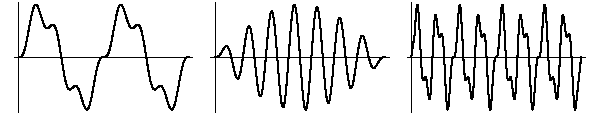
\includegraphics[width=\textwidth]{ode/inhomogeneous/non_res_forcing}
      \end{center}
      \caption{Non-resonant forcing.}
      \label{non_res_forcing}
    \end{figure}

    For $\lambda = 1$, we have
    \begin{align*}
      y       &= \frac{1}{2} \int_0^t \big( \cos(t - 2 \tau) - \cos(tau) \big) \,\dd \tau\\
      &= \frac{1}{2} \left[ - \frac{1}{2} \sin( t - 2 \tau) - \tau \cos t
      \right]_0^t
    \end{align*}
    \begin{equation}
      \label{res_forcing_soln}
      \boxed{
        y = \frac{1}{2} \left( \sin t - t \cos t \right).
        }
    \end{equation}
    The solution has both a periodic and a transient term.
    This solution is plotted in Figure~\ref{non_res_forcing}
    on the interval $t \in [0,16 \pi]$.
    \begin{figure}[tb!]
      \begin{center}
        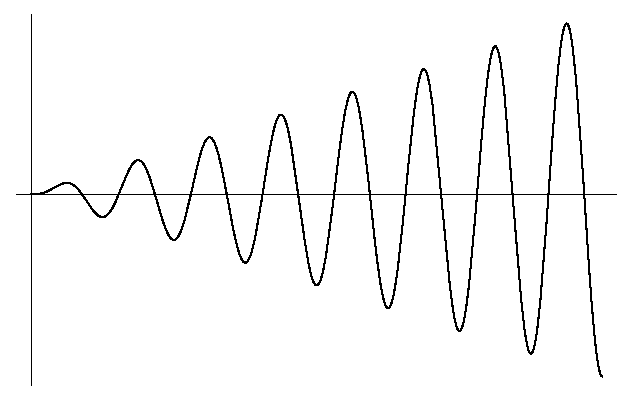
\includegraphics[width=0.3\textwidth]{ode/inhomogeneous/res_forcing}
      \end{center}
      \caption{Resonant forcing.}
      \label{res_forcing}
    \end{figure}

    Note that we can derive (\ref{res_forcing_soln}) from
    (\ref{non_res_forcing_soln}) by
    taking the limit as $\lambda \to 0$.
    \begin{align*}
      \lim_{\lambda \to 1} \frac{ \sin(\lambda t) - \lambda \sin t }{ 1 - \lambda^2 }
      &= \lim_{\lambda \to 1} \frac{ t \cos(\lambda t) - \sin t }
      {- 2 \lambda} \\
      &= \frac{1}{2} \left( \sin t - t \cos t \right)
    \end{align*}
  \end{enumerate}
\end{Solution}






%%222222222222222222222222222222222222222222222222222222222222222222222222222
\begin{Solution}
  \label{solution y+p2y+p1y+p0y=f}
  Let $y_1$, $y_2$ and $y_3$ be linearly independent homogeneous solutions
  to the differential equation
  \[ L[y] = y''' + p_2 y'' + p_1 y' + p_0 y = f(x). \]
  We will look for a particular solution of the form
  \[ y_p = u_1 y_1 + u_2 y_2 + u_3 y_3. \]
  Since the $u_j$'s are undetermined functions, we are free to impose two
  constraints.  We choose the constraints to simplify the algebra.
  \begin{align*}
    u_1' y_1 + u_2' y_2 + u_3' y_3 &= 0 \\
    u_1' y_1'+ u_2' y_2'+ u_3' y_3'&= 0
  \end{align*}
  Differentiating the expression for $y_p$,
  \begin{align*}
    y_p'    &= u_1' y_1 + u_1 y_1' + u_2' y_2 + u_2 y_2' + u_3' y_3 + u_3 y_3' \\
    &= u_1 y_1' + u_2 y_2' + u_3 y_3' \\
    y_p''   &= u_1' y_1' + u_1 y_1'' + u_2' y_2' + u_2 y_2'' 
    + u_3' y_3' + u_3 y_3'' \\
    &= u_1 y_1'' + u_2 y_2'' + u_3 y_3'' \\
    y_p'''  &= u_1' y_1'' + u_1 y_1''' + u_2' y_2'' + u_2 y_2''' 
    + u_3' y_3'' + u_3 y_3''' 
  \end{align*}
  Substituting the expressions for $y_p$ and its derivatives into the 
  differential equation,
  \begin{align*}
    &u_1' y_1'' + u_1 y_1''' + u_2' y_2'' + u_2 y_2''' + u_3' y_3'' + u_3 y_3'''
    + p_2 (u_1 y_1'' + u_2 y_2'' + u_3 y_3'')
    + p_1 (u_1 y_1' + u_2 y_2' + u_3 y_3') \\
    &\qquad + p_0 (u_1 y_1 + u_2 y_2 + u_3 y_3) = f(x) 
  \end{align*}
  \begin{gather*}
    u_1' y_1'' + u_2' y_2'' + u_3' y_3'' + u_1 L[y_1] + u_2 L[y_2] + u_3 L[y_3]
    = f(x) \\
    u_1' y_1'' + u_2' y_2'' + u_3' y_3'' = f(x).
  \end{gather*}
  With the two constraints, we have the system of equations,
  \begin{align*}
    u_1' y_1 + u_2' y_2 + u_3' y_3 &= 0 \\
    u_1' y_1'+ u_2' y_2'+ u_3' y_3'&= 0 \\
    u_1' y_1'' + u_2' y_2'' + u_3' y_3'' &= f(x)
  \end{align*}
  We solve for the $u_j'$ using Kramer's rule.
  \[ u_1' = \frac{(y_2 y_3' - y_2' y_3)f(x)}{W(x)}, \quad
  u_2' = -\frac{(y_1 y_3' - y_1' y_3)f(x)}{W(x)}, \quad
  u_3' = \frac{(y_1 y_2' - y_1' y_2)f(x)}{W(x)} \]
  Here $W(x)$ is the Wronskian of $\{y_1, y_2, y_3\}$.  Integrating the 
  expressions for $u_j'$, the particular solution is
  \[ \boxed{ y_p = y_1 \int \frac{(y_2 y_3' - y_2' y_3) f(x)}{W(x)}\,\dd x
    + y_2 \int \frac{(y_3 y_1' - y_3' y_1) f(x)}{W(x)}\,\dd x
    + y_3 \int \frac{(y_1 y_2' - y_1' y_2) f(x)}{W(x)}\,\dd x. }\]
\end{Solution}


%%-----------------------------------------------------------------------------
\begin{large}
  \noindent
  \textbf{Green Functions}
\end{large}



%% y'' = f(x), \quad y(-\infty) = y'(-\infty) = 0.
\begin{Solution}
  \label{solution y=f y=y=0}
  We consider the Green function problem
  \[
  G'' = f(x), \quad G(-\infty|\xi) = G'(-\infty|\xi) = 0.
  \]
  The homogeneous solution is $y = c_1 + c_2 x$.  The homogeneous solution
  that satisfies the boundary conditions is $y = 0$.  Thus the Green function
  has the form
  \[
  G(x|\xi) = 
  \begin{cases}
    0 &x < \xi, \\
    c_1 + c_2 x & x > \xi.
  \end{cases}
  \]
  The continuity and jump conditions are then
  \[
  G(\xi^+|\xi) = 0, \quad G'(\xi^+|\xi) = 1.
  \]
  Thus the Green function is
  \[
  G(x|\xi) = 
  \begin{cases}
    0 &x < \xi, \\
    x - \xi & x > \xi
  \end{cases}
  = (x - \xi) H(x - \xi).
  \]
  The solution of the problem 
  \[
  y'' = f(x), \quad y(-\infty) = y'(-\infty) = 0.
  \]
  is
  \begin{gather*}
    y = \int_{-\infty}^\infty f(\xi) G(x|\xi) \,\dd \xi \\
    y = \int_{-\infty}^\infty f(\xi) (x - \xi) H(x - \xi) \,\dd \xi \\
    \boxed{
      y = \int_{-\infty}^x f(\xi) (x - \xi) \,\dd \xi 
      }
  \end{gather*}
  We differentiate this solution to verify that it satisfies the differential
  equation.
  \begin{gather*}
    y' = \left[ f(\xi) (x - \xi) \right]_{\xi = x} 
    + \int_{-\infty}^x \frac{\partial}{\partial x} \left( f(\xi) (x - \xi) 
    \right) \,\dd \xi 
    = \int_{-\infty}^x f(\xi) \,\dd \xi \\
    y'' = \left[ f(\xi) \right]_{\xi = x} = f(x)
  \end{gather*}
\end{Solution}






%%111111111111111111111111111111111111111111111111111111111111111111111111111
\begin{Solution}
  \label{solution y+1xy-1x2y=x2}
  Since we are dealing with an Euler equation, we substitute $y = x^\lambda$
  to find the homogeneous solutions.
  \begin{gather*}
    \lambda(\lambda-1) + \lambda - 1 = 0 \\
    (\lambda-1)(\lambda+1) = 0 \\
    y_1 = x, \qquad y_2 = \frac{1}{x}
  \end{gather*}

  \paragraph{Variation of Parameters.}
  The Wronskian of the homogeneous solutions is
  \[W(x) = 
  \begin{vmatrix}
    x       & 1/x \\
    1       & -1/x^2
  \end{vmatrix}
  = -\frac{1}{x} - \frac{1}{x} = -\frac{2}{x}.
  \]
  A particular solution is
  \begin{align*}
    y_p     &= - x \int \frac{x^2(1/x)}{-2/x}\,\dd x 
    + \frac{1}{x} \int \frac{x^2 x}{-2/x}\,\dd x \\
    &= -x \int -\frac{x^2}{2}\,\dd x 
    + \frac{1}{x} \int -\frac{x^4}{2}\,\dd x \\
    &= \frac{x^4}{6} - \frac{x^4}{10} \\
    &= \frac{x^4}{15}.
  \end{align*}
  The general solution is
  \[y = \frac{x^4}{15} + c_1 x + c_2 \frac{1}{x}.\]
  Applying the initial conditions,
  \begin{alignat*}{2}
    y(0) &= 0 \quad &\to \quad c_2 &= 0 \\
    y'(0) &= 0 \quad &\to \quad c_1 &= 1.
  \end{alignat*}
  Thus we have the solution 
  \[ \boxed{y = \frac{x^4}{15} + x.} \]



  \paragraph{Green Function.}
  Since this problem has both an inhomogeneous term in the differential equation
  and inhomogeneous boundary conditions, we separate it into the two problems
  \begin{alignat*}{2}
    &u'' + \frac{1}{x} u' - \frac{1}{x^2} u = x^2, &\qquad &u(0) = u'(0) = 0, \\
    &v'' + \frac{1}{x} v' - \frac{1}{x^2} v = 0, &\qquad &v(0) = 0,\ v'(0) = 1.
  \end{alignat*}

  First we solve the inhomogeneous differential equation with the homogeneous
  boundary conditions.  The Green function for this problem satisfies
  \[ L[G(x|\xi)] = \delta(x-\xi), \quad G(0|\xi) = G'(0|\xi) = 0. \]
  Since the Green function must satisfy the
  homogeneous boundary conditions, it has the form
  \[ G(x|\xi) = 
  \begin{cases}
    0 \quad &\mathrm{for}\ x < \xi \\
    c x + d/x \quad &\mathrm{for}\ x > \xi.
  \end{cases}
  \]
  From the continuity condition,
  \[ 0 = c \xi + d / \xi.\]
  The jump condition yields
  \[ c - d/ \xi^2 = 1.\]
  Solving these two equations, we obtain
  \[ G(x|\xi) = 
  \begin{cases}
    0 \quad &\mathrm{for}\ x < \xi \\
    \frac{1}{2} x - \frac{\xi^2}{2 x} \quad &\mathrm{for}\ x > \xi
  \end{cases}
  \]
  Thus the solution is
  \begin{align*}
    u(x)    &= \int_0^\infty G(x|\xi) \xi^2\,\dd \xi \\
    &= \int_0^x \left(\frac{1}{2} x - \frac{\xi^2}{2 x}\right)\xi^2\,\dd \xi\\
    &= \frac{1}{6}x^4 - \frac{1}{10}x^4 \\
    &= \frac{x^4}{15}.
  \end{align*}

  Now to solve the homogeneous differential equation with inhomogeneous 
  boundary conditions.
  The general solution for $v$ is
  \[ v = c x + d / x. \]
  Applying the two boundary conditions gives
  \[ v = x.\]

  Thus the solution for $y$ is
  \[ \boxed{y = x + \frac{x^4}{15}.} \]
\end{Solution}












%%333333333333333333333333333333333333333333333333333333333333333333333333333333
\begin{Solution}
  \label{solution continuity y+p2y+p1y+p0y=f}
  The Green function satisfies
  \[
  G'''(x|\xi) + p_2(x) G''(x|\xi) + p_1(x) G'(x|\xi) + p_0(x) G(x|\xi) 
  = \delta(x-\xi).
  \]
  First note that only the $G'''(x|\xi)$ term can have a delta function 
  singularity.  If a lower derivative had a delta function type singularity, 
  then $G'''(x|\xi)$ would be more singular than a delta function and there
  would be no other term in the equation to balance that behavior.  Thus we see 
  that $G'''(x|\xi)$ will have a delta function singularity; $G''(x|\xi)$ will
  have a jump discontinuity; $G'(x|\xi)$ will be continuous at $x=\xi$.
  Integrating the differential equation from $\xi^-$ to $\xi^+$ yields
  \[
  \int_{\xi^-}^{\xi^+} G'''(x|\xi) \,\dd x
  = \int_{\xi^-}^{\xi^+} \delta(x-\xi) \,\dd x
  \]
  \[
  G''(\xi^+|\xi) - G''(\xi^-|\xi) = 1.
  \]
  Thus we have the three continuity conditions:
  \begin{align*}
    G''(\xi^+|\xi) &= G''(\xi^-|\xi) + 1 \\
    G'(\xi^+|\xi) &= G'(\xi^-|\xi) \\
    G(\xi^+|\xi) &= G(\xi^-|\xi) 
  \end{align*}
\end{Solution}















%%44444444444444444444444444444444444444444444444444444444444444444444444444444
\begin{Solution}
  \label{solution x2y-2xy+2y=e-x}
  \textbf{Variation of Parameters.}
  Consider the problem
  \[ 
  x^2 y'' - 2 x y' + 2 y = \e^{-x}, \qquad y(1) = 0, \quad y'(1) = 1. 
  \]
  Previously we showed that two homogeneous solutions are
  \[ 
  y_1 = x, \qquad y_2 = x^2. 
  \]
  The Wronskian of these solutions is
  \[ 
  W(x) =
  \begin{vmatrix}
    x       &       x^2     \\
    1       &       2x
  \end{vmatrix}
  = 2x^2 - x^2 = x^2.
  \]
  In the variation of parameters formula, we will choose $1$ as the lower
  bound of integration.  (This will simplify the algebra in applying the
  initial conditions.)
  \begin{align*}
    y_p     &= -x \int_1^x \frac{\e^{-\xi} \xi^2}{\xi^4}\,\dd \xi + x^2 \int_1^x
    \frac{\e^{-\xi} \xi}{\xi^4}\,\dd \xi \\
    &= -x \int_1^x \frac{\e^{-\xi}}{\xi^2} \,\dd \xi 
    + x^2 \int_1^x \frac{\e^{-\xi}}{\xi^3} \,\dd \xi \\
    &= -x \left(\e^{-1}-\frac{\e^{-x}}{x} 
      - \int_1^x \frac{\e^{-\xi}}{\xi} \,\dd \xi \right)
    + x^2 \left( \frac{\e^{-x}}{2x} - \frac{\e^{-x}}{2x^2}
      + \frac{1}{2}\int_1^x \frac{\e^{-\xi}}{\xi} \,\dd \xi \right)\\
    &= -x \e^{-1} + \frac{1}{2} (1+x) \e^{-x} 
    + \left(\frac{x+x^2}{2}\right) 
    \int_1^x \frac{\e^{-\xi}}{\xi} \,\dd \xi
  \end{align*}
  If you wanted to, you could write the last integral in terms of exponential
  integral functions.

  The general solution is
  \[ 
  y = c_1 x + c_2 x^2  -x \e^{-1} + \frac{1}{2} (1+x) \e^{-x} 
  + \left(x+\frac{x^2}{2}\right) \int_1^x \frac{\e^{-\xi}}{\xi} \,\dd \xi
  \]
  Applying the boundary conditions,
  \begin{alignat*}{3}
    &y(1) = 0 &\qquad &\to &\qquad &c_1 + c_2 = 0 \\
    &y'(1) = 1 &\qquad &\to &\qquad &c_1 + 2 c_2 = 1,
  \end{alignat*}
  we find that $c_1 = -1$, $c_2 = 1$.

  Thus the solution subject to the initial conditions is
  \[ 
  \boxed{ 
    y = -(1+\e^{-1})x + x^2 + \frac{1}{2} (1+x) \e^{-x} 
    + \left(x+\frac{x^2}{2}\right) \int_1^x \frac{\e^{-\xi}}{\xi} \,\dd \xi
    }
  \]

  \textbf{Green Functions.}
  The solution to the problem is $y=u+v$ where 
  \[
  u'' - \frac{2}{x} u' + \frac{2}{x^2} u = \frac{\e^{-x}}{x^2}, \qquad
  u(1)=0, \quad u'(1)=0,
  \]
  and
  \[
  v'' - \frac{2}{x} v' + \frac{2}{x^2} v = 0, \qquad v(1)=0, \quad v'(1)=1.
  \]
  The problem for $v$ has the solution
  \[
  v = -x + x^2.
  \]
  The Green function for $u$ is
  \[
  G(x|\xi) = H(x-\xi) u_\xi(x)
  \]
  where
  \[
  u_\xi(\xi) = 0, \quad \mathrm{and} \quad u_\xi'(\xi)=1.
  \]
  Thus the Green function is
  \[
  G(x|\xi) = H(x-\xi) \left(-x + \frac{x^2}{\xi} \right).
  \]
  The solution for $u$ is then
  \begin{align*}
    u       &= \int_1^\infty G(x|\xi) \frac{\e^{-\xi}}{\xi^2} \,\dd \xi \\
    &= \int_1^x \left(-x + \frac{x^2}{\xi} \right) 
    \frac{\e^{-\xi}}{\xi^2} \,\dd \xi \\
    &= -x \e^{-1} + \frac{1}{2}(1+x)\e^{-x} + \left(x+\frac{x^2}{2}\right)
    \int_1^x \frac{\e^{-\xi}}{\xi} \,\dd \xi.
  \end{align*}
  Thus we find the solution for $y$ is
  \[ 
  \boxed{ 
    y = -(1+\e^{-1})x + x^2 + \frac{1}{2} (1+x) \e^{-x} 
    + \left(x+\frac{x^2}{2}\right) \int_1^x \frac{\e^{-\xi}}{\xi} \,\dd \xi
    }
  \]
\end{Solution}





%% Find the Green function for \[ y'' - y = f(x), \qquad y'(0) = y(1) = 0. \]
\begin{Solution}
  \label{solution y-y=f y0=y1=0}
  The differential equation for the Green function is
  \[
  G'' - G = \delta(x - \xi), \qquad G_x(0|\xi) = G(1|\xi) = 0.
  \]
  Note that $\cosh(x)$ and $\sinh(x-1)$ are homogeneous solutions that satisfy
  the left and right boundary conditions, respectively.  The Wronskian of 
  these two solutions is
  \begin{align*}
    W(x)    &= \begin{vmatrix} \cosh(x) & \sinh(x-1) \\ \sinh(x) & \cosh(x-1)
    \end{vmatrix} \\
    &= \cosh(x) \cosh(x-1) - \sinh(x) \sinh(x-1) \\
    &= \frac{1}{4} \left( \left( \e^x + \e^{-x} \right)
      \left( \e^{x-1} + \e^{-x+1} \right) 
      - \left( \e^x - \e^{-x} \right)
      \left( \e^{x-1} - \e^{-x+1} \right) \right) \\
    &= \frac{1}{2} \left( \e^1 + \e^{-1} \right) \\
    &= \cosh(1).
  \end{align*}
  The Green function for the problem is then
  \[
  G(x|\xi) = \frac{ \cosh(x_<) \sinh(x_> - 1) }{ \cosh(1) },
  \]
  \[
  \boxed{
    G(x|\xi) = \begin{cases}
      \frac{ \cosh(x) \sinh(\xi-1) }{ \cosh(1) } &\mathrm{for}\ 0 \leq x \leq \xi, \\
      \frac{ \cosh(\xi) \sinh(x-1) }{ \cosh(1) } &\mathrm{for}\ \xi \leq x \leq 1. \\
    \end{cases}
    }
  \]
\end{Solution}





%% Find the Green function for \[ y'' - y = f(x), \qquad y(0) = y(\infty) = 0.\]
\begin{Solution}
  \label{solution y-y=f y0=yinf=0}
  The differential equation for the Green function is
  \[
  G'' - G = \delta(x - \xi), \qquad G(0|\xi) = G(\infty|\xi) = 0.
  \]
  Note that $\sinh(x)$ and $\e^{-x}$ are homogeneous solutions that satisfy
  the left and right boundary conditions, respectively.  The Wronskian of 
  these two solutions is
  \begin{align*}
    W(x)    &= \begin{vmatrix} \sinh(x) & \e^{-x} \\ \cosh(x) & - \e^{-x}
    \end{vmatrix} \\
    &= - \sinh(x) \e^{-x} - \cosh(x) \e^{-x} \\
    &= - \frac{1}{2} \left( \e^x - \e^{-x} \right) \e^{-x}
    - \frac{1}{2} \left( \e^x + \e^{-x} \right) \e^{-x} \\
    &= -1
  \end{align*}
  The Green function for the problem is then
  \[
  G(x|\xi) = - \sinh(x_<) \e^{-x_>}
  \]
  \[
  \boxed{
    G(x|\xi) = \begin{cases}
      - \sinh(x) \e^{-\xi} &\mathrm{for}\ 0 \leq x \leq \xi, \\
      - \sinh(\xi) \e^{-x} &\mathrm{for}\ \xi \leq x \leq \infty. \\
    \end{cases}
    }
  \]
\end{Solution}







%% Find the Green function for each of the following:
\begin{Solution}
  \label{solution xu+u=f}

  $\phantom{a}$  %% Force a line break

  \begin{itemize}
    %%
  \item[a)]
    The Green function problem is
    \[
    x G''(x|\xi) + G'(x|\xi) = \delta(x-\xi), \quad G(0|\xi)\ \mathrm{bounded,}\ 
    G(1|\xi) = 0.
    \]
    First we find the homogeneous solutions of the differential equation.
    \[
    x y'' + y' = 0
    \]
    This is an exact equation.
    \[
    \frac{\dd}{\dd x} [ x y' ] = 0
    \]
    \[
    y' = \frac{c_1}{x}
    \]
    \[
    y = c_1 \log x + c_2
    \]
    The homogeneous solutions $y_1 = 1$ and $y_2 = \log x$ satisfy the left and
    right boundary conditions, respectively.  The Wronskian of these solutions
    is
    \[
    W(x) = \begin{vmatrix} 1 & \log x \\ 0 & 1/x \end{vmatrix}
    = \frac{1}{x}.
    \]
    The Green function is
    \[
    G(x|\xi) = \frac{ 1 \cdot \log x_> }{ \xi (1/\xi) },
    \]
    \[
    \boxed{
      G(x|\xi) = \log x_>.
      }
    \]
    %%
  \item[b)]
    The Green function problem is
    \[
    G''(x|\xi) - G(x|\xi) = \delta(x-\xi), \quad
    G(-a|\xi) = G(a|\xi) = 0.
    \]
    $\{\e^x, \e^{-x}\}$ and $\{ \cosh x, \sinh x\}$ are both linearly independent
    sets of homogeneous solutions.  $\sinh(x+a)$ and $\sinh(x-a)$ are homogeneous
    solutions that satisfy the left and right boundary conditions, respectively.
    The Wronskian of these two solutions is,
    \begin{align*}
      W(x)    &= \begin{vmatrix} \sinh(x+a) & \sinh(x-a) \\
        \cosh(x+a) & \cosh(x-a) \end{vmatrix} \\
      &= \sinh(x+a) \cosh(x-a) - \sinh(x-a) \cosh(x+a)  \\
      &= \sinh(2 a)
    \end{align*}
    The Green function is
    \[
    \boxed{
      G(x|\xi) = \frac{ \sinh(x_< + a) \sinh(x_> - a) }{ \sinh(2 a) }.
      }
    \]
    %%
  \item[c)]
    The Green function problem is
    \[
    G''(x|\xi) - G(x|\xi) = \delta(x - \xi), \quad
    G(x|\xi)\ \mathrm{bounded as}\ |x| \to \infty.
    \]
    $\e^{x}$ and $\e^{-x}$ are homogeneous solutions that satisfy the left 
    and right boundary conditions, respectively.  The Wronskian of these solutions
    is
    \[
    W(x) = \begin{vmatrix} \e^x & \e^{-x} \\ \e^x & - \e^{-x} \end{vmatrix}
    = -2.
    \]
    The Green function is
    \[
    G(x|\xi) = \frac{ \e^{x_<} \e^{- x_>} }{ -2 },
    \]
    \[
    \boxed{
      G(x|\xi) = - \frac{1}{2} \e^{x_< - x_>}.
      }
    \]
    %%
  \item[d)]
    The Green function from part (b) is,
    \[
    G(x|\xi) = \frac{ \sinh(x_< + a) \sinh(x_> - a) }{ \sinh(2 a) }.
    \]
    We take the limit as $a \to \infty$.
    \begin{align*}
      \lim_{a \to \infty} \frac{ \sinh(x_< + a) \sinh(x_> - a) }{ \sinh(2 a) }
      &= \lim_{a \to \infty} \frac{ 
        \left( \e^{x_< + a} - \e^{-x_< - a} \right)
        \left( \e^{x_> - a} - \e^{-x_> + a} \right) }
      { 2 \left( \e^{2 a} - \e^{-2 a} \right) } \\
      &= \lim_{a \to \infty} \frac{ -\e^{x_< - x_>} + \e^{x_< + x_> - 2a} 
        + \e^{-x_< - x_> - 2 a} - \e^{-x_< + x_> - 4a } }
      { 2 - 2 \e^{-4 a} } \\
      &= - \frac{ \e^{x_< - x_>} }{ 2 }
    \end{align*}
    Thus we see that the solution from part (b) approaches the solution from 
    part (c) as $a \to \infty$.
  \end{itemize}
\end{Solution}











%% For what values of $\lambda$ does the problem 
\begin{Solution}
  \label{solution y+lambday=f}
  \begin{enumerate}
  \item
    The problem,
    \[
    y'' + \lambda y = f(x), \quad y(0) = y(\pi) = 0,
    \]
    has a Green function if and only if it has a unique solution.  This 
    inhomogeneous problem has a unique solution if and only if the homogeneous
    problem has only the trivial solution.

    First consider the case $\lambda = 0$.  We find the general solution of the 
    homogeneous differential equation.
    \[
    y = c_1 + c_2 x
    \]
    Only the trivial solution satisfies the boundary conditions.  The problem
    has a unique solution for $\lambda = 0$.

    Now consider non-zero $\lambda$.  We find the general solution of the 
    homogeneous differential equation.
    \[
    y = c_1 \cos \left( \sqrt{\lambda} x \right)
    + c_2 \sin \left( \sqrt{\lambda} x \right).
    \]
    The solution that satisfies the left boundary condition is
    \[
    y = c \sin \left( \sqrt{\lambda} x \right).
    \]
    We apply the right boundary condition and find nontrivial solutions.
    \begin{gather*}
      \sin \left( \sqrt{\lambda} \pi \right) = 0
      \\
      \lambda = n^2, \quad n \in \mathbb{Z}^+
    \end{gather*}
    Thus the problem has a unique solution for all complex $\lambda$ except
    $\lambda = n^2$, $n \in \mathbb{Z}^+$.

    Consider the case $\lambda = 0$.  We find solutions of the homogeneous equation 
    that satisfy the left and right boundary conditions, respectively.
    \[
    y_1 = x, \qquad y_2 = x - \pi.
    \]
    We compute the Wronskian of these functions.
    \[
    W(x) = 
    \begin{vmatrix}
      x & x - \pi \\
      1 & 1 
    \end{vmatrix}
    = \pi.
    \]
    The Green function for this case is
    \[
    G(x|\xi) = \frac{x_< (x_> - \pi)}{\pi}.
    \]
    We consider the case $\lambda \neq n^2$, $\lambda \neq 0$.  
    We find the solutions of the homogeneous equation that satisfy 
    the left and right boundary conditions, respectively.
    \[
    y_1 = \sin \left( \sqrt{\lambda} x \right), \qquad 
    y_2 = \sin \left( \sqrt{\lambda} (x - \pi) \right).
    \]
    We compute the Wronskian of these functions.
    \[
    W(x) = 
    \begin{vmatrix}
      \sin \left( \sqrt{\lambda} x \right) &
      \sin \left( \sqrt{\lambda} (x - \pi) \right) \\
      \sqrt{\lambda} \cos \left( \sqrt{\lambda} x \right) &
      \sqrt{\lambda} \cos \left( \sqrt{\lambda} (x - \pi) \right)
    \end{vmatrix}
    = \sqrt{\lambda} \sin \left( \sqrt{\lambda} \pi \right)
    \]
    The Green function for this case is
    \[
    G(x|\xi) = \frac{ \sin \left( \sqrt{\lambda} x_< \right)
      \sin \left( \sqrt{\lambda} (x_> - \pi ) \right) }
    { \sqrt{\lambda} \sin \left( \sqrt{\lambda} \pi \right) }.
    \]

  \item
    Now we consider the problem
    \[
    y'' + 9 y = 1 + \alpha x, \quad y(0) = y(\pi) = 0.
    \]
    The homogeneous solutions of the problem
    are constant multiples of $\sin(3 x)$.  
    Thus for each value of $\alpha$, the problem either has no solution or an
    infinite number of solutions.  There will be an infinite number
    of solutions if the inhomogeneity $1 + \alpha x$ is orthogonal to the
    homogeneous solution $\sin(3 x)$ and no solution otherwise.
    \[
    \int_0^\pi (1 + \alpha x) \sin(3 x) \,\dd x = \frac{\pi \alpha + 2}{3}
    \]
    The problem has a solution only for $\alpha = - 2/\pi$.  For this case 
    the general solution of the inhomogeneous differential equation is
    \[
    y = \frac{1}{9} \left( 1 - \frac{2 x}{\pi} \right) + c_1 \cos(3 x) 
    + c_2 \sin(3 x).
    \]
    The one-parameter family of solutions that satisfies the boundary 
    conditions is
    \[
    y = \frac{1}{9} \left( 1 - \frac{2 x}{\pi} - \cos(3 x) \right) + c \sin(3 x).
    \]

  \item
    For $\lambda = n^2$, $n \in \mathbb{Z}^+$, $y = \sin(n x)$ is a solution of the
    homogeneous equation that satisfies the boundary conditions.
    Equation~\ref{eqn y'' + lambda y = f, y = y = 0} has a (non-unique) 
    solution only if $f$ is orthogonal to $\sin(n x)$.
    \[
    \int_0^\pi f(x) \sin(n x) \,\dd x = 0
    \]
    The modified Green function satisfies
    \[
    G'' + n^2 G = \delta(x - \xi) - \frac{ \sin(n x) \sin(n \xi) }{ \pi / 2 }.
    \]
    We expand $G$ in a series of the eigenfunctions.
    \[
    G(x|\xi) = \sum_{k = 1}^\infty g_k \sin(k x)
    \]
    We substitute the expansion into the differential equation to determine the
    coefficients.  This will not determine $g_n$.  We choose $g_n = 0$, which is 
    one of the choices that will make the modified Green function symmetric in
    $x$ and $\xi$.
    \begin{gather*}
      \sum_{k = 1}^\infty g_k \left( n^2 - k^2 \right) \sin(k x) 
      = \frac{2}{\pi} \sum_{\substack{k = 1 \\ k \neq n}}^\infty \sin(k x) \sin(k \xi)
      \\
      \boxed{
        G(x|\xi) = \frac{2}{\pi} \sum_{\substack{k = 1 \\ k \neq n}}^\infty 
        \frac{ \sin(k x) \sin(k \xi) }{ n^2 - k^2 }
        }
    \end{gather*}
    The solution of the inhomogeneous problem is
    \[
    y(x) = \int_0^\pi f(\xi) G(x|\xi) \,\dd \xi.
    \]
  \end{enumerate}
\end{Solution}









%% Show that the inhomogeneous boundary value problem:
\begin{Solution}
  \label{solution Lu=pu+qu=f}
  We separate the problem for $u$ into the two problems:
  \begin{gather*}
    L v \equiv (p v')' + q v = f(x), \quad a < x < b, 
    \quad v(a) = 0, \quad v(b) = 0 \\
    L w \equiv (p w')' + q w = 0, \quad a < x < b, 
    \quad w(a) = \alpha, \quad w(b) = \beta 
  \end{gather*}
  and note that the solution for $u$ is $u = v + w$.  

  The problem for $v$ has the solution,
  \[
  v = \int_a^b g(x;\xi) f(\xi) \,\dd \xi,
  \]
  with the Green function,
  \[
  g(x;\xi) = \frac{v_1(x_<) v_2(x_>)}{ p(\xi) W(\xi) } \equiv
  \begin{cases}
    \frac{v_1(x) v_2(\xi)}{ p(\xi) W(\xi) } &\mathrm{for}\ a \leq x \leq \xi, \\
    \frac{v_1(\xi) v_2(x)}{ p(\xi) W(\xi) } &\mathrm{for}\ \xi \leq x \leq b. \\
  \end{cases}
  \]
  Here $v_1$ and $v_2$ are homogeneous solutions that respectively satisfy 
  the left and right homogeneous boundary conditions.

  Since $g(x;\xi)$ is a solution of the homogeneous equation for $x \neq \xi$,
  $g_\xi(x;\xi)$ is a solution of the homogeneous equation for $x \neq \xi$.
  This is because for $x \neq \xi$, 
  \[
  L \left[ \frac{\partial}{\partial \xi} g \right] = \frac{\partial}{\partial \xi} L[g]
  = \frac{\partial}{\partial \xi} \delta(x-\xi) = 0.
  \]
  If $\xi$ is outside of the domain, $(a,b)$, then $g(x;\xi)$ and
  $g_\xi(x;\xi)$ are homogeneous solutions on that domain.  In particular
  $g_\xi(x;a)$ and $g_\xi(x;b)$ are homogeneous solutions,
  \[
  L \left[ g_\xi(x;a) \right] = L \left[ g_\xi(x;b) \right] = 0.
  \]
  Now we use the definition of the Green function and $v_1(a) = v_2(b) = 0$
  to determine simple expressions for these homogeneous solutions.
  \begin{align*}
    g_\xi(x;a) &= \frac{ v_1'(a) v_2(x) }{ p(a) W(a) }
    - \frac{ (p'(a) W(a) + p(a) W'(a)) v_1(a) v_2(x) }{ (p(a) W(a))^2 } \\
    &= \frac{ v_1'(a) v_2(x) }{ p(a) W(a) } \\
    &= \frac{ v_1'(a) v_2(x) }{ p(a) (v_1(a) v_2'(a) - v_1'(a) v_2(a)) } \\
    &= - \frac{ v_1'(a) v_2(x) }{ p(a) v_1'(a) v_2(a) } \\
    &= - \frac{ v_2(x) }{ p(a) v_2(a) } 
  \end{align*}
  We note that this solution has the boundary values,
  \[
  g_\xi(a;a) = - \frac{ v_2(a) }{ p(a) v_2(a) } = - \frac{1}{p(a)}, \qquad
  g_\xi(b;a) = - \frac{ v_2(b) }{ p(a) v_2(a) } = 0.
  \]
  We examine the second solution.
  \begin{align*}
    g_\xi(x;b) &= \frac{ v_1(x) v_2'(b) }{ p(b) W(b) }
    - \frac{ (p'(b) W(b) + p(b) W'(b)) v_1(x) v_2(b) }{ (p(b) W(b))^2 } \\
    &= \frac{ v_1(x) v_2'(b) }{ p(b) W(b) } \\
    &= \frac{ v_1(x) v_2'(b) }{ p(b) (v_1(b) v_2'(b) - v_1'(b) v_2(b)) } \\
    &= \frac{ v_1(x) v_2'(b) }{ p(b) v_1(b) v_2'(b) } \\
    &= \frac{ v_1(x) }{ p(b) v_1(b) } 
  \end{align*}
  This solution has the boundary values,
  \[
  g_\xi(a;b) = \frac{ v_1(a) }{ p(b) v_1(b) } = 0, \qquad
  g_\xi(b;b) = \frac{ v_1(b) }{ p(b) v_1(b) } = \frac{1}{p(b)}.
  \]
  Thus we see that the solution of 
  \[
  L w = (p w')' + q w = 0, \quad a < x < b, 
  \quad w(a) = \alpha, \quad w(b) = \beta,
  \]
  is
  \[
  w = - \alpha p(a) g_\xi(x;a) + \beta p(b) g_\xi(x;b).
  \]
  Therefore the solution of the problem for $u$ is
  \[
  \boxed{
    u = \int_a^b g(x;\xi) f(\xi) \,\dd \xi 
    - \alpha p(a) g_\xi(x;a) + \beta p(b) g_\xi(x;b).
    }
  \]
\end{Solution}








%% Green function for reduced wave equation by image method.
\begin{Solution}
  \label{solution u-k2u=f}
  Figure~\ref{helmholtz1am1} shows a plot of $G(x;1)$ and $G(x;-1)$ for $k=1$.

  \begin{figure}[tb!]
    \begin{center}
      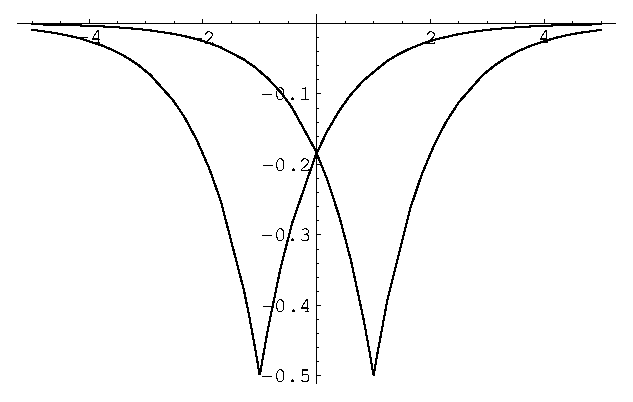
\includegraphics[width=0.4\textwidth]{ode/inhomogeneous/helmholtz1am1}
    \end{center}
    \caption{The Green functions.}
    \label{helmholtz1am1}
  \end{figure}

  First we consider the boundary condition $u(0) = 0$.  Note that the solution of
  \[
  G'' - k^2 G = \delta(x - \xi) - \delta(x+\xi), |G(\pm\infty;\xi)| < \infty,
  \]
  satisfies the condition $G(0;\xi) = 0$.  Thus the Green function which 
  satisfies $G(0;\xi) = 0$ is
  \[
  G(x;\xi) = - \frac{1}{2k} \e^{-k |x-\xi|} + \frac{1}{2k} \e^{-k |x+\xi|}.
  \]
  Since $x,\xi > 0$ we can write this as
  \begin{align*}
    G(x;\xi) &= - \frac{1}{2k} \e^{-k |x-\xi|} + \frac{1}{2k} \e^{-k (x+\xi)} \\
    &= \begin{cases}
      - \frac{1}{2k} \e^{-k (\xi-x)} + \frac{1}{2k} \e^{-k (x+\xi)},
      &\mathrm{for}\ x < \xi \\
      - \frac{1}{2k} \e^{-k (x-\xi)} + \frac{1}{2k} \e^{-k (x+\xi)},
      &\mathrm{for}\ \xi < x 
    \end{cases} \\
    &= \begin{cases}
      - \frac{1}{k} \e^{-k \xi} \sinh(k x), &\mathrm{for}\ x < \xi \\
      - \frac{1}{k} \e^{-k x} \sinh(k \xi), &\mathrm{for}\ \xi < x 
    \end{cases} \\
  \end{align*}
  \[
  \boxed{
    G(x;\xi) = - \frac{1}{k} \e^{-k x_>} \sinh(k x_<)
    }
  \]

  Now consider the boundary condition $u'(0) = 0$.  Note that the solution of
  \[
  G'' - k^2 G = \delta(x-\xi) + \delta(x+\xi), \quad |G(\pm\infty;\xi)| < \infty,
  \]
  satisfies the boundary condition $G'(x;\xi) = 0$.  Thus the Green function is
  \[
  G(x;\xi) = - \frac{1}{2k} \e^{-k |x-\xi|} - \frac{1}{2k} \e^{-k |x+\xi|}.
  \]
  Since $x,\xi > 0$ we can write this as
  \begin{align*}
    G(x;\xi) &= - \frac{1}{2k} \e^{-k |x-\xi|} - \frac{1}{2k} \e^{-k (x+\xi)} \\
    &= \begin{cases}
      - \frac{1}{2k} \e^{-k (\xi-x)} - \frac{1}{2k} \e^{-k (x+\xi)},
      &\mathrm{for}\ x < \xi \\
      - \frac{1}{2k} \e^{-k (x-\xi)} - \frac{1}{2k} \e^{-k (x+\xi)},
      &\mathrm{for}\ \xi < x 
    \end{cases} \\
    &= \begin{cases}
      - \frac{1}{k} \e^{-k \xi} \cosh(k x), &\mathrm{for}\ x < \xi \\
      - \frac{1}{k} \e^{-k x} \cosh(k \xi), &\mathrm{for}\ \xi < x 
    \end{cases} \\
  \end{align*}
  \[
  \boxed{
    G(x;\xi) = - \frac{1}{k} \e^{-k x_>} \cosh(k x_<)
    }
  \]

  The Green functions which satisfy $G(0;\xi) = 0$ and $G'(0;\xi) = 0$ 
  are shown in Figure~\ref{helmholtz1}.  We plot $G(x;1)$ and $G(x;-1)$.

  \begin{figure}[tb!]
    \begin{center}
      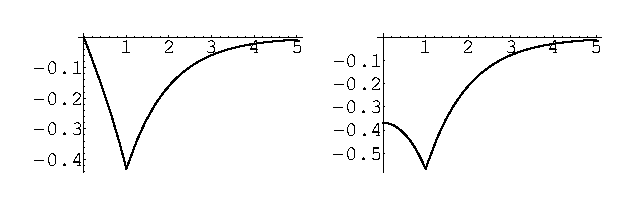
\includegraphics[width=0.5\textwidth]{ode/inhomogeneous/helmholtz1}
    \end{center}
    \caption{The Green functions.}
    \label{helmholtz1}
  \end{figure}
\end{Solution}






%% y'' - a^2 y = f(x), \quad y(0) = y'(L) = 0.
\begin{Solution}
  \label{solution y-a2y=f}
  \begin{enumerate}
    %%
    %%
  \item
    The Green function satisfies
    \[
    g'' - a^2 g = \delta(x - \xi), \quad g(0;\xi) = g'(L;\xi) = 0.
    \]
    We can write the set of homogeneous solutions as
    \[
    \left\{ \e^{a x}, \e^{-a x} \right\}\ \mathrm{or}\ 
    \left\{ \cosh(a x), \sinh(a x) \right\}.
    \]
    The solutions that respectively satisfy the left and right boundary conditions 
    are
    \[
    u_1 = \sinh(a x), \quad u_2 = \cosh(a (x - L)).
    \]
    The Wronskian of these solutions is
    \[
    W(x) = 
    \begin{pmatrix}
      \sinh(a x) & \cosh(a(x-L)) \\
      a \cosh(a x) & a \sinh(a(x-L))
    \end{pmatrix}
    = -a \cosh(a L).
    \]
    Thus the Green function is
    \[
    \boxed{
      g(x;\xi) = 
      \begin{cases}
        - \frac{ \sinh(a x) \cosh(a (\xi-L)) }{ a \cosh(a L) } 
        &\mathrm{for}\ x \leq \xi, \\
        - \frac{ \sinh(a \xi) \cosh(a (x-L)) }{ a \cosh(a L) } 
        &\mathrm{for}\ \xi \leq x. 
      \end{cases}
      =
      - \frac{ \sinh(a x_<) \cosh(a (x_> -L)) }{ a \cosh(a L) }.
      }
    \]
    %%
    %%
  \item
    We take the limit as $L \to \infty$.
    \begin{align*}
      g(x;\xi)
      &= \lim_{L \to \infty} - \frac{ \sinh(a x_<) \cosh(a (x_> -L)) }
      { a \cosh(a L) } \\
      &= \lim_{L \to \infty} - \frac{ \sinh(a x_<) }{ a }
      \frac{ \cosh( a x_> ) \cosh( a L ) 
        - \sinh( a x_> ) \sinh( a L ) }{ \cosh(a L) } \\
      &= - \frac{ \sinh(a x_<) }{ a }
      ( \cosh( a x_> ) - \sinh( a x_> ) ) 
    \end{align*}
    \[
    \boxed{
      g(x;\xi) = - \frac{1}{a} \sinh(a x_<) \e^{-a x_>} 
      }
    \]
    The solution of 
    \[
    y'' - a^2 y = \e^{-x}, \quad y(0) = y'(\infty) = 0
    \]
    is
    \begin{align*}
      y       &= \int_0^\infty g(x;\xi) \e^{-\xi} \,\dd \xi \\
      &= - \frac{1}{a} \int_0^\infty \sinh(a x_<) \e^{-a x_>} \e^{-\xi} \,\dd \xi \\
      &= - \frac{1}{a} \left( 
        \int_0^x \sinh(a \xi) \e^{-a x} \e^{- \xi} \,\dd \xi
        + \int_x^\infty \sinh(a x) \e^{-a \xi} \e^{-\xi} \,\dd \xi 
      \right) \\
      \intertext{We first consider the case that $a \neq 1$.}
      &= - \frac{1}{a} \left( 
        \frac{ \e^{-a x} }{a^2 - 1} \left( -a + \e^{-x} 
          ( a \cosh(a x) + \sinh(a x) ) \right)
        + \frac{1}{a+1} \e^{-(a+1) x} \sinh(a x)
      \right) \\
      &= \frac{ \e^{-a x} - \e^{-x} }{ a^2 - 1 }
    \end{align*}
    For $a = 1$, we have
    \begin{align*}
      y       &= - \left( \frac{1}{4} \e{-x} \left( -1 + 2 x + \e^{-2 x} \right)
        + \frac{1}{2} \e^{-2 x} \sinh(x) \right) \\
      &= - \frac{1}{2} x \e^{-x}.
    \end{align*}
    Thus the solution of the problem is
    \[
    \boxed{
      y = 
      \begin{cases}
        \frac{ \e^{-a x} - \e^{-x} }{ a^2 - 1 } &\mathrm{for}\ a \neq 1, \\
        - \frac{1}{2} x \e^{-x} &\mathrm{for}\ a = 1.
      \end{cases}
      }
    \]
    We note that this solution satisfies the differential equation and 
    the boundary conditions.
  \end{enumerate}
\end{Solution}







}



\raggedbottom
%%=============================================================================
\pagebreak
\flushbottom
\section{Quiz}


\begin{QuizProblem}
  \label{quiz problem y'' - y = f}
  Find the general solution of 
  \[
  y'' - y = f(x),
  \]
  where $f(x)$ is a known function.

  \quizsolution{y'' - y = f}
\end{QuizProblem}










\raggedbottom
%%=============================================================================
\pagebreak
\flushbottom
\section{Quiz Solutions}


\begin{QuizSolution}
  \label{quiz solution y'' - y = f}
  \[
  y'' - y = f(x)
  \]
  We substitute $y = \e^{\lambda x}$ into the homogeneous differential equation.
  \begin{gather*}
    y'' - y = 0 
    \\
    \lambda^2 \e^{\lambda x} - \e^{\lambda x} = 0 
    \\
    \lambda = \pm 1
  \end{gather*}
  The homogeneous solutions are $\e^{x}$ and $\e^{-x}$.  The Wronskian of 
  these solutions is
  \[
  \begin{vmatrix}
    \e^x & \e^{-x} 
    \\
    \e^x & - \e^{-x}
  \end{vmatrix}
  = - 2.
  \]
  We find a particular solution with variation of parameters.
  \[
  y_p = - \e^x \int \frac{\e^{-x} f(x)}{-2} \,\dd x
  + \e^{-x} \int \frac{\e^x f(x)}{-2} \,\dd x
  \]
  The general solution is
  \[
  y = c_1 \e^x + c_2 \e^{-x}
  - \e^x \int \frac{\e^{-x} f(x)}{-2} \,\dd x
  + \e^{-x} \int \frac{\e^x f(x)}{-2} \,\dd x.
  \]
\end{QuizSolution}







\raggedbottom
